% !TeX program = PdfLaTeX

\documentclass[a4paper,12pt,oneside,openright]{book}


%--------------------------------------------------------------------------------------------------------------------------------------------
%PACKAGES
%--------------------------------------------------------------------------------------------------------------------------------------------

%Document settings
\usepackage[utf8]{inputenc}
\usepackage[T1]{fontenc}
\usepackage[full]{textcomp}
\usepackage[italian, english]{babel}
%Questi comandi servono per settare i linguaggi
\providecommand{\csletcs}[2]{%
\expandafter\let\csname#1\expandafter\endcsname\csname#2\endcsname}
\newcommand{\equivUC}[3][\def]{%
\expandafter#1\csname#2\expandafter\endcsname\expandafter{%
\csname#3\endcsname}}
\newcommand{\UPCASElang}[1]{
\uppercase{\def\temp{#1}}
\csletcs{l@\temp}{l@#1}
\equivUC{date\temp}{date#1}
\equivUC{captions\temp}{captions#1}
\equivUC{extras\temp}{extras#1}
\equivUC{noextras\temp}{noextras#1}
\equivUC[\edef]{\temp hyphenmins}{#1hyphenmins}
}
\UPCASElang{english}
\UPCASElang{italian}
\usepackage{csquotes}
\usepackage{indentfirst}    
\usepackage{geometry}
\geometry{a4paper, top=20mm, bottom=20mm, left=35mm, right=20mm } %MARGINI 
\raggedbottom  %Per non riempire tutta la pagina stirando il testo. puo lasciare spazi vuoti alla fine di una pagina
\linespread{1} 

%Other useful packages
\usepackage[TM]{ar} %aspect ratio symbol. To use it --> \AR
\usepackage[usenames,dvipsnames]{xcolor}
\usepackage{pgfplots}
\pgfplotsset{compat=1.13}
\usepackage{caption}
\usepackage{graphicx}
\usepackage{tabularx}
\usepackage{longtable}
\usepackage{multicol}
\usepackage{multirow}
\usepackage{setspace}
\usepackage{booktabs}
\usepackage[intlimits]{mathtools}
\usepackage{siunitx}
\usepackage{subfig}
\usepackage{rotating}
\usepackage{float}
\usepackage{fancyhdr}
\usepackage{floatflt}
\usepackage{xcolor}
\usepackage{colortbl}
\usepackage{wrapfig}
\usepackage{lipsum}
\usepackage[nouppercase, swapnames]{frontespizio}
\usepackage{adjustbox}
\usepackage{booktabs}
\usepackage{amsmath}
\usepackage{cancel}
\usepackage{listings}
\usepackage{lipsum}
\usepackage{courier}
\usepackage{xcolor}
\usepackage{relsize}
\usepackage{titlesec} 
\usepackage{appendix}
\usepackage{xspace}
\usepackage{floatflt}
\usepackage{varioref}
\usepackage{tabulary}
\usepackage[backend=biber]{biblatex}
\addbibresource{bibliography.bib}
\definecolor{grigio_chiaro}{gray}{0.85}
%\usepackage[autostyle,italian=guillemets]{csquotes}
%\usepackage[backend=biber]{biblatex}

%---------------------------------------------------------------
% Listing settings
%----------------------------------------------------------------

\DeclareCaptionFormat{listing}{{\textwidth+17pt\relax\centering}\par\vskip1pt#1#2#3}
\captionsetup[lstlisting]{format=listing,singlelinecheck=false, justification=centering, margin=0pt, font={rm},labelsep=space,labelfont=bf}


\definecolor{light-gray}{gray}{0.97}
\lstset{frameround=fttt}
\lstset{language=Java}
\lstset{%
backgroundcolor=\color{light-gray}}
\lstset{basicstyle=\scriptsize\ttfamily,
keywordstyle=\color{blue}\bfseries,
commentstyle=\color{OliveGreen},
stringstyle=\color{blue},
showstringspaces=true}


\lstset{framextopmargin=50pt,frame=bottomline}

\usepackage { fancyhdr }
\newcommand {\fncyblank }{\fancyhf {}}
\newenvironment { abstract }%
{\cleardoublepage \fncyblank \null \vfill \begin { center }%
\bfseries \abstractname \end { center }}%
{\vfill \null }

\newenvironment{abstract}%
{\cleardoublepage%
  \thispagestyle{empty}%
  \null \vfill\begin{center}%
  \bfseries \huge\scshape  \abstractname \end{center}}%
{\vfill\null}

\newcommand{\myChapterHeadingColorMix}{%
  %blue!65!black
  gray!0!black%
}

\newcommand{\myChapterHeadingColor}{%
  %blue!65!black
  blue!0!black%
}


\usepackage{fancyhdr}


\renewcommand{\chaptermark}[1]{\markboth{#1}{}}
\lhead {{\bfseries \chaptername \ \thechapter} \; \leftmark}
\chead{}
\rhead{ \thepage }
\lfoot{}
\cfoot{}
\rfoot{\scriptsize Manuela Ruocco - Development of a Java-Based Framework for Aircraft Preliminary Design}
\renewcommand{\headrulewidth}{0.4pt}
\renewcommand{\footrulewidth}{0.4pt}


\fancypagestyle{pippo}{%
\pagestyle{fancy}
\lhead{}
\chead{}
\rhead{ \thepage }
\lfoot{}
\cfoot{}
\rfoot{\scriptsize Manuela Ruocco - Development of a Java Application for Aircraft Preliminary Design}
\renewcommand{\headrulewidth}{0.4pt}
\renewcommand{\footrulewidth}{0.4pt}

}


\titleformat{\chapter}[display]
  {  \bfseries \Large}
  {\filleft \huge { \bfseries{\chaptertitlename}}   \lapbox[6pt]{\width} 
 \ \colorbox{\myChapterHeadingColorMix}{\color{white}\Huge \strut {\thechapter}}}
  {3ex}
  {\titlerule\vspace{2ex}\filright}
  [\vspace{2ex}{\titlerule[2pt]}]



%------------------------------------------------------------------------------------------
% One of the last package to be loaded must be hyperref

\usepackage[%
            %dvipdfmx,%dvips,%
            %pdfborder = 0 0 1,
            baseurl= http://,
            colorlinks=true,%
            linkcolor=black,% black
            citecolor=black% black
            ]{hyperref}
\usepackage{cleveref}
%\usepackage{createspace}


%\addbibresource%
%%   [datatype=bibtex]%
%   {Tesi.bib}% extension required

%*************************************************************************************
% BIBLATEX SETTINGS POST-HYPERREF

\bibliography{Tesi_Bibliography}% with biblatex
\defbibheading{myBibliography}[\bibname]{\chapter*{\centering#1}
   %\markboth{#1}{#1}
   \markboth{}{}
}

\DeclareCiteCommand{\citetitle}{}{\printfield{title}}{;}{}


% http://tex.stackexchange.com/questions/83440/inputenc-error-unicode-char-u8-not-set-up-for-use-with-latex
%\DeclareUnicodeCharacter{00A0}{ }
%\DeclareUnicodeCharacter{00A0}{~}

%*************************************************************************************


 % queste sono alcune impostazioni gia settate

% nuovi comandi
\newcommand\nbvspace[1][3]{\vspace*{\stretch{#1}}}
\newcommand\nbstretchyspace{\spaceskip0.5em plus 0.25em minus 0.25em}

%--------------------------------------------------------------------------------------------------------------------------------------------
%BEGIN DOCUMENT
%--------------------------------------------------------------------------------------------------------------------------------------------
\begin{document}

%--------------------------------------------------------------------------------------------------------------------------------------------
%COPERTINA/FRONTESPIZIO
%--------------------------------------------------------------------------------------------------------------------------------------------

%FRONTESPIZIO
\begin{frontespizio}
\Universita {Napoli Federico II}
\Divisione {Scuola Politecnica e delle Scienze di Base}
\Corso [Laurea Triennale]{Ingegneria Aerospaziale}
\Logo [3cm]{immagini/Logo_UNINA.pdf}
\Titoletto {Tesi di Laurea Triennale \\ in \\ Ingegneria Aerospaziale}
\Titolo {Assessment of minimum unstick speed \\ of a complete Aircraft using JPAD \\ (Java toolchain Program  for Aircraft Design)}
%\Sottotitolo {Wing Aerodynamic Analysis Module,\\ Aircraft Longitudinal Static Stability Module }
\Candidato {Bruno Spoti \\ Matricola N35/2018}
%\Relatore {Prof. Ing. Fabrizio Nicolosi }
\Relatore {Prof. Ing. Agostino De Marco}
\Correlatore{Ing. Manuela Ruocco}
\Annoaccademico {2017/2018}
\end{frontespizio}

% -----------------------------------------------------------------------------------------
%                                                                    INSERIRE PAGINA BIANCA
% -----------------------------------------------------------------------------------------

\newpage\null\thispagestyle{empty}\newpage\thispagestyle{empty}

% -----------------------------------------------------------------------------------------
%                                                                    D E D I C A  (non in indice)
% -----------------------------------------------------------------------------------------

\null\vspace{\stretch{1}}
\begin{flushright}
\textit{Sono sempre i sogni a dare forma al mondo,\\ sono sempre i sogni a fare la realtà.}
\end{flushright}
\vspace{\stretch{2}}\null
\newpage\null\thispagestyle{empty}

% -----------------------------------------------------------------------------------------
%                                                                   PREFAZIONE
% -----------------------------------------------------------------------------------------

\selectlanguage{english}
\begin{abstract}
The purpose of this Thesis work is to introduce the features and the potenciality of ADOpT ({\itshape Aircraft Design and Optimization Tool}), a java-based framework concieved as a fast and efficient tool useful as support in the preliminary design phases of an aircraft, and during its optimizaton process.\\
The ADOpT development originates in the Departement of Industrial Engineering of University of Naples ``Federico II'', where is still in development. At present this tool is capable to perform a multi-disciplinary analysis of an aircraft whose data can be entered by the user, with an XML, or loaded into memory. The ultimate goal of ADOpT is to carry out an optimization process where the analysis are cyclically repeated in order to optimize some parameters while keeping others in fixed limits.
Currently the software is able to esimate the aircraft weight breackdown, the center of gravity location, calculate some aerodynamic parameters and estimate the performance. All these types of estimates can be usually performed using several interchangeable analysis methods, comparable and interchangeable. 
It is also provided a static longitudinal stability analysis, take-off and landing performances and the generation of Payload Range chart.\\
ADOpT can be used from the command line or with a dedicated graphical user interface (GUI). The GUI allows the user to have an immediate feedback about the aircraft features when changing the input parameters, to manage multiple aircraft simultaneously and compare them side by side, and to view a 3D CAD model of the aircraft. \\
The ADOpT potentiality, in the world of research or in industry, are remarkable and the software strengths are a considerable computing speed and flexibility, with an user-friendly GUI.\\ \\
The structure of this thesis work has as ultimate goal to provide a comprehensive overview about ADOpT and, at the same time, it is intended to be a developer's manual. The first chapters provide a complete software overview paying particular attention at actual features and future goals.
Following chapters introduce  some case of study and the results achieved. At the beginning of each chapter is exposed the theoretical background, afterwards there is a description of the Java architecture and, at the end is reported the Test class used for the analysis and its results.

\end{abstract}

\selectlanguage{italian}
\begin{abstract}

Lo scopo che il presente lavoro di Tesi auspica raggiungere è quello di presentare le capacità possedute e le potenzialità future di ADOpT, un software scritto in Java che si configura come uno strumento veloce ed efficiente per il supporto nella fase di progetto preliminare di un velivolo e per la sua ottimizzazione. \\
Lo sviluppo di ADOpT ({\itshape Aircraft Design and Optimization Tool}) nasce all' interno del Dipartimento di Ingegneria Industriale dell' Università degli Studi di Napoli Federico II, ove è tutt'ora in fase di progresso. Il software è attualmente in grado di svolgere una parziale analisi multi-disciplinare di un velivolo i cui dati sono immessi dall' utente tramite XML o caricati in memoria. La linea guida dello sviluppo del software porta verso l'implementazione di un processo di ottimizzazione nel quale le analisi sono ciclicamente ripetute al fine di ottimizzare alcuni parametri mantenendone altri all' interno di limiti imposti.\\
Attualmente ADOpT è in grado di effettuare una completa stima dei pesi, valutare la posizione del baricentro, calcolare un notevole numero di parametri aerodinamici e caratteristiche di performance. La stima di ciascun parametro può essere effettuata tramite diversi metodi implementati, tra di loro confrontabili ed intercambiabili. Inoltre è prevista un' analisi di stabilità statica, prestazioni di decollo ed atterraggio e la generazione del diagramma  {\itshape Payload Range}.\\
ADOpT può essere utilizzato sia in modalità {\itshape batch}, ossia da riga di comando, che tramite interfaccia grafica. Tale duplice scelta consente di ottenere le migliori prestazioni sia nei processi di analisi, ove la GUI consente di avere un immediato riscontro grafico, sia nei processi di ottimizzazione.\\
Dunque le potenzialità di ADOpT nel mondo della ricerca od anche in quello industriale sono senza dubbio notevoli e il software gioca i suoi punti di forza in un' elevata flessibilità e una notevole rapidità di calcolo, senza dimenticare e una {\itshape user-friendly} interfaccia grafica. \\ \\

L' organizzazione di questo lavoro di Tesi è stata studiata per cercare di fornire una completezza di esposizione, ma allo stesso tempo risultare un utile manuale per lo sviluppatore. I primi capitoli forniscono una visione globale del software con particolare attenzione alle funzionalità presenti e alle scelte effettuate.
I capitoli che seguono presentano una panoramica su alcune funzionalità di ADOpT con i relativi casi di studio e i risultati ottenuti dalle analisi. Per ogni capitolo viene preliminarmente fornita una visione globale circa la teoria alla base dei metodi implementati, seguita dalla descrizione delle classi e dei metodi  relativi in Java ed è, infine, riportato il codice della {\itshape Test Class} implementata per lo svolgimento dell' analisi con i relativi risultati.





%La tesi descrive lo sviluppo diadopt,, un'applicazione scritta in linguaggio Java concepita per essere uno strumento veloce, affidabile e di semplice utilizzo per le fasi di sviluppo concettuale e preliminare di un velivolo da trasporto. Lo scopo finale del programma è effettuare un'analisi multidisciplinare di una configurazione definita dall'utente e successivamente alterarla in modo da ottenerne una ottimizzata. Il dominio di ricerca di tale configurazione è definito dall'utente tramite un apposito insieme di parametri.
%
%Allo stato attuale il programma effettua la stima dei pesi dei principali componenti di un velivolo, valuta la posizione del baricentro, i principali parametri aerodinamici e alcune derivate di stabilità. La stima di ciascun parametro può essere generalmente effettuata tramite diversi metodi tra loro intercambiabili. Il carico aerodinamico sull'ala, in particolare, è stato stimato tramite un metodo numerico tratto danasa blackwell. Molta attenzione è stata in generale dedicata alla validazione dei risultati forniti dall'applicazione.
%
%ADOpT può essere usato sia da riga di comando sia tramite un'apposita interfaccia grafica (GUI). Quest'ultima fornisce un riscontro immediato riguardo il cambiamento delle prestazioni del velivolo nel momento in cui l'utente modifica uno o più parametri di input; inoltre permette di gestire più velivoli (o più configurazioni dello stesso velivolo) simultaneamente, di confrontarne le caratteristiche e di visualizzarne il modello CAD. Questo è generato tramite la libreria opencascade e può essere salvato su file in modo da poterlo usare in altri applicativi.
%
%Per quanto riguarda i files di input e di output, l'applicazione accetta files in formato XML (eXtensible Markup Language) contenenti la configurazione del velivolo e può esportare i risulati sia in formato XML sia in formato XLS. I file XML di uscita possono esssere successivamente re-importati e quindi modificati tramite l'interfaccia grafica. L'applicazione è stata sviluppata facendo largo uso delle ultime caratteristiche del linguaggio Java introdotte da Oracle nel 2014 con la versione 8; questa include, tra l'altro, la piattaforma JavaFX che è stata usata per costruire il visualizzatore del modello CAD.
\end{abstract}
\selectlanguage{english} 
\newpage
% !TeX program = PdfLaTeX
% !TeX root = ../Main.tex

\renewcommand{\abstractname}{Sommario}
\begin{abstract}
Lo scopo di questo lavoro di tesi è implementare una specifica routine Java per valutare la
VMU di un aereo completo. Questo è stato fatto implementando nuove ca\-rat\-te\-ri\-sti\-che in JPAD
(Java toolchain Program for Aircraft Design), un framework scritto in Java concepito come un veloce ed
efficiente strumento a supporto nelle fasi preliminari di progettazione di un aereo e durante il suo
processo di ottimizzazione. \\
Lo sviluppo di JPAD ha origine nel Dipartimento di Ingegneria Industriale dell'Università di Napoli "Federico II", dove è ancora in corso.
JPAD è un software dotato di un'interfaccia grafica (GUI) e, al momento, è in grado di eseguire un'analisi multidisciplinare
di un aeromobile i cui dati possono essere inseriti dall'utente, con un file XML, o caricati in memoria. \\

La struttura di questo lavoro di tesi è articolata in 3 capitoli e 1 appendice. \\
Prima di tutto, viene presentata la struttura di JPAD. \\
Il secondo capitolo riguarda un background teorico il quale, partendo da una breve introduzione della velocità di decollo, si sposterà sulla spiegazione dell'effetto suolo e sulla sua implementazione. Questo capitolo termina con la presentazione della VMU. \\
Il terzo capitolo riguarda un caso studio eseguito su un turboelica regionale di 130 passeggeri, riguardante le caratteristiche aerodinamiche, i dispositivi di ipersostentazione e l'effetto suolo sia sulla curva di portanza dell'ala che sull'angolo di downwash. \\
Lo sviluppo delle nuove funzionalità Java, in JPAD, è stato fatto prendendo in con\-si\-de\-ra\-zio\-ne la possibilità di ulteriori sviluppi per consentire l'introduzione di nuovi metodi. \\
Alla fine, nell'appendice A, viene mostrato come digitalizzare un grafico, creare un set di dati in formato .h5 e impostare la classe che legge di database in JPAD.
\end{abstract}

% -----------------------------------------------------------------------------------------
%                                                                   INDICE  (non in indice)
% -----------------------------------------------------------------------------------------

\tableofcontents 
\listoffigures
% -----------------------------------------------------------------------------------------
%                                                                 C A P I T O L I
% -----------------------------------------------------------------------------------------

\chapter{Introduction to JPAD}
\label{ch1}

Nowadays the preliminary design phase of an aircraft is becoming very challenging due to the need for more demanding requirements which deals with different fields of applications. In this perspective, there is a certain need for simple design tools both in aircraft industries and academic research groups which can perform fast and reliable multi-disciplinary analyses and optimizations.

This chapter provides a comprehensive overview of JPAD (Java toolchain of Programs for Aircraft Design) \cite{paper:JPAD}, a Java-based open-source library conceived as a fast and efficient tool useful as support in the preliminary design phases of an aircraft, and during its optimization process. The library has been completely realized at the Department of Industrial Engineering of the University of Naples “Federico II” where is still in development.

One of the main features of JPAD lies in the smart management of both the aircraft parametric model, which is conceived as a set of interconnected and parameterized components, and the available analyses. The library has been developed with the purpose of simplify the composition of the input file for the user and doing fast analysis with a satisfying grade of accuracy. The following section will focus on the description of the software structure and its main advantages. Another key point is the possibility to easily interface JPAD with other external tools in order to achieve a higher level of accuracy.

The JPAD library is an alternative to a plethora of similar software tools, both freeware and commercial \cite{AAA} \cite{Piano5} \cite{RDS}. Most of these tools have an important history, and many of them have been in use for decades. Some of them were conceived with poor software design criteria, have a rigid textual input and come with no visualization features. This is the main reason why JPAD has been developed paying a lot of attention to simplicity and flexibility. Moreover, it has been conceived as an open-source tool.

% --------------------------------------------------------------------------------------------------------------------------------------------
% SEZIONE 1
% --------------------------------------------------------------------------------------------------------------------------------------------
\section{Software structure}
\label{sec1.1}

To achieve a clear input file organization a considerable study has been done. The result is an input structure composed by different XML files with the purpose to allow users to easily manage all data needed to execute the desired analyses. In figure~\vref{JPADSchematicFlowChart} the entire structure of the software is schematized. It is possible to clearly note that there are two main blocks: input and core.

\begin{figure}[htbp] 
\centering
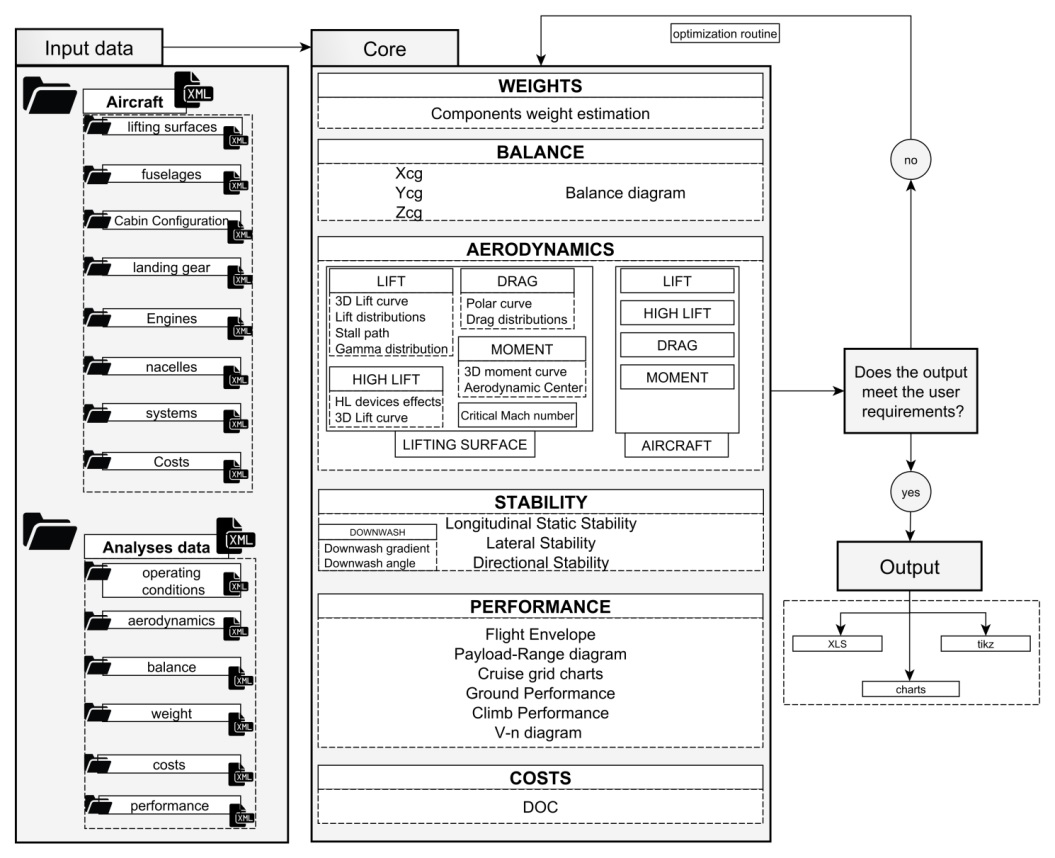
\includegraphics[height=0.45\textheight]{Immagini/Capitolo1/1_1-JPADSchematicFlowChart}
\caption[JPAD schematic flow-chart] {JPAD schematic flow-chart}
\label{JPADSchematicFlowChart}
\end{figure}

\begin{figure}[htbp] 
\centering
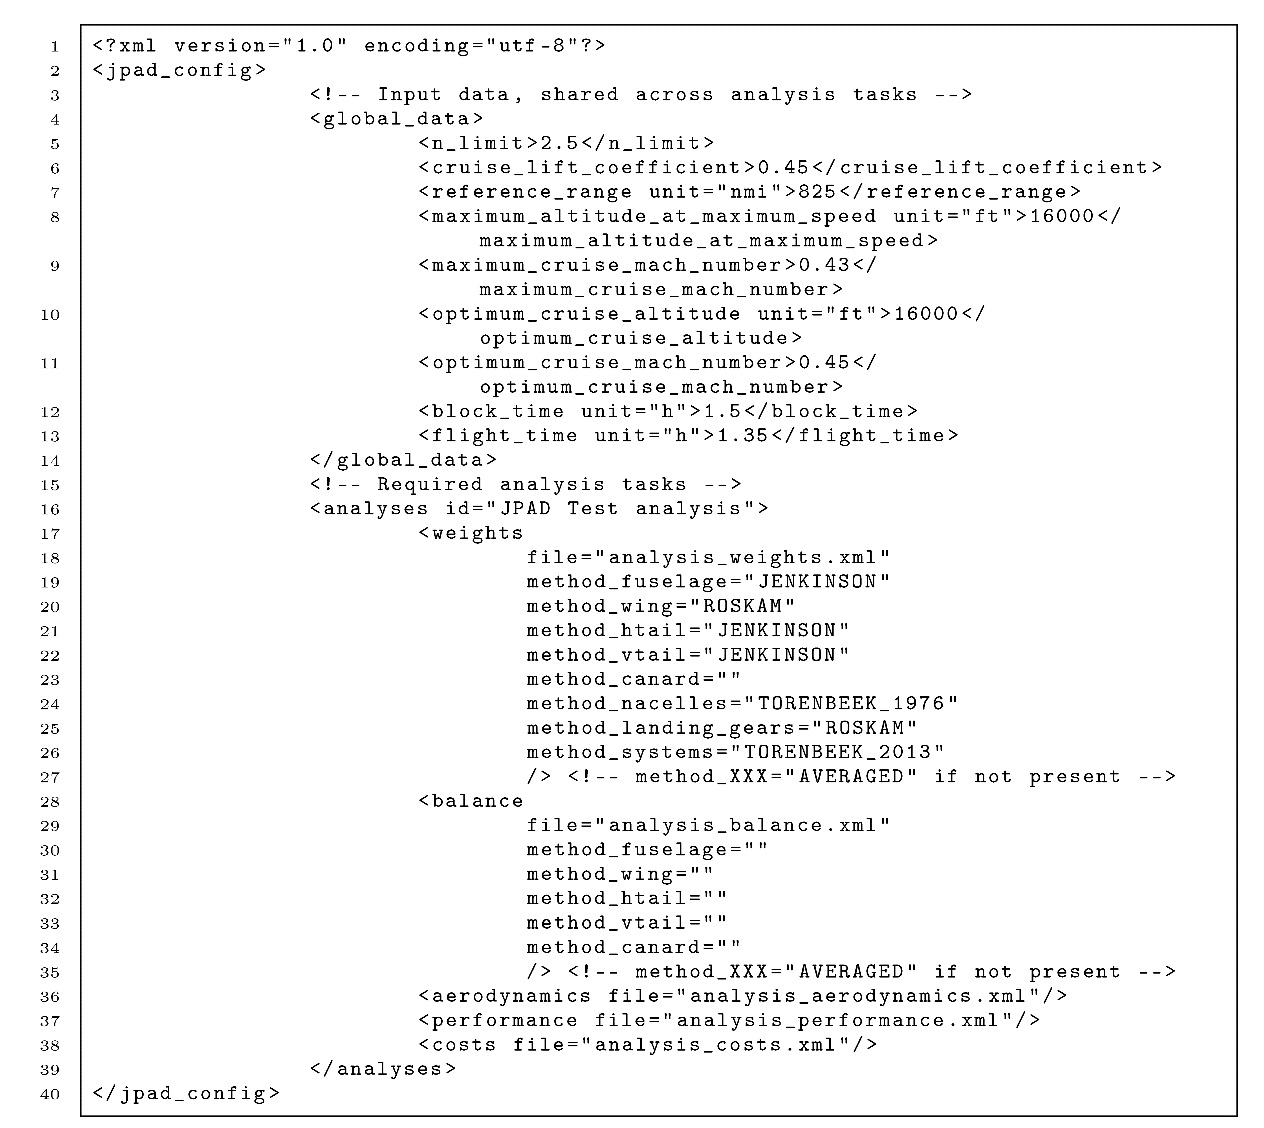
\includegraphics[height=0.45\textheight]{Immagini/Capitolo1/1_2-AnExampleOfTheAnalysisXmlFile}
\caption[Example of analysis.xml file] {An example of the analysis.xml file}
\label{AnExampleOfTheAnalysisXmlFile}
\end{figure}

\begin{figure}[htbp] 
\centering
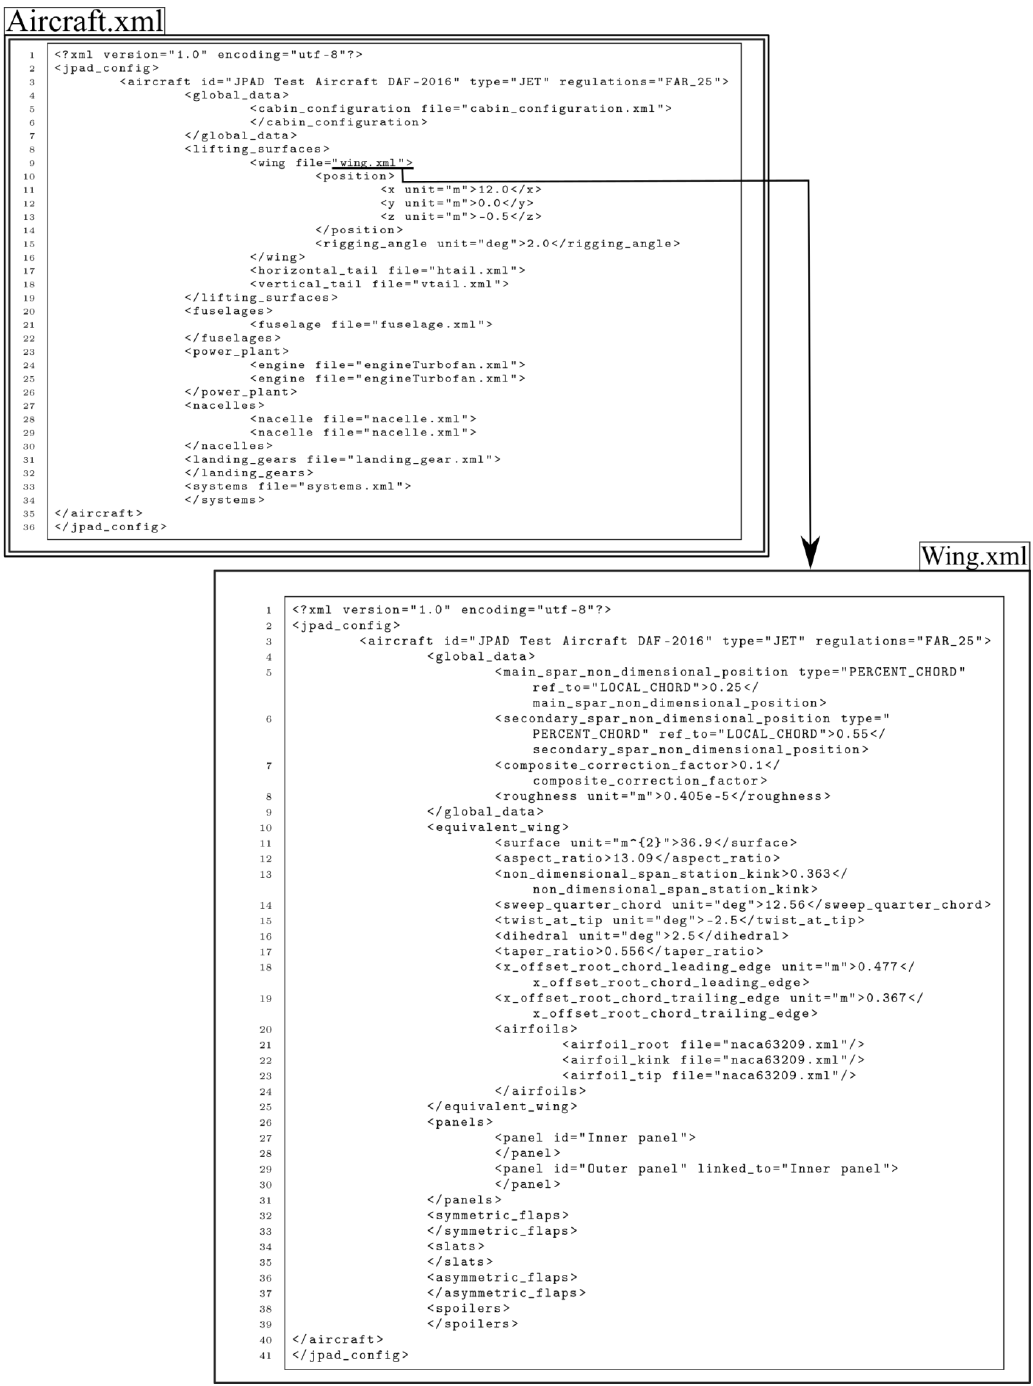
\includegraphics[width=\textwidth]{Immagini/Capitolo1/1_3-AnExtractFromAGeneralAircraftXmlInputFile}
\caption[Extract from general Aircraft.xml input file] {An extract from a general Aircraft.xml input file}
\label{AnExtractFromAGeneralAircraftXmlInputFile}
\end{figure}

The input block is defined by two main parts: aircraft and analyses definitions. The first one defines the aircraft model in parametric way using a main file (Aircraft.xml, see figure~\ref{AnExtractFromAGeneralAircraftXmlInputFile}) which collects all the components, linking them to their related XML file (i.e. fuselage.xml, vtail.xml, and so on) which contains all geometrical data.

The second one defines all necessary data for each analysis presents into core module (see figure~\ref{AnExampleOfTheAnalysisXmlFile}). Since the aircraft model contains only geometrical data, it is necessary to define several further data referred to each analysis. \\

The structure described above allows to generate different aircrafts, or different configurations of the same model, combining different components. The possibility to generate a series of different aircrafts in a simple and fast way, allows to easily perform comparisons between these latter. For example, assuming different wings and engines, it is possible to estimate the effects that some design parameters have on a specific output. Figure~\vref{FAR-25} shows how the FAR-25 take-off field length behaves with different values of the wing surface and the engine static thrust at fixed aircraft maximum take-off weight. This feature plays also a key role in the optimization process described in figure~\ref{JPADSchematicFlowChart}.

\begin{figure}[htbp] 
\centering
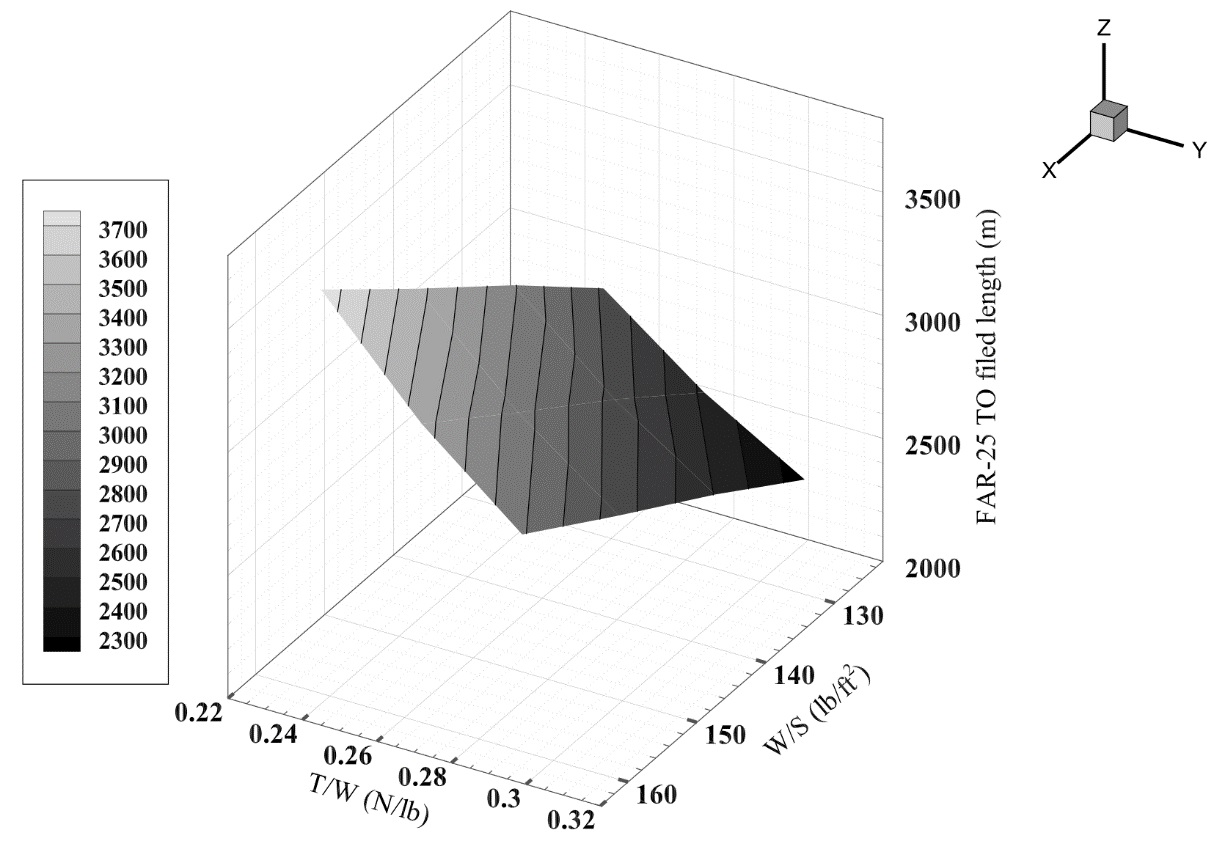
\includegraphics[width=\textwidth]{Immagini/Capitolo1/1_4-FAR-25TakeOffFieldLengthAtDifferentWingLoadingsAndThrustWeightRatios}
\caption[FAR-25 take-off field length at different $W/S_\text W$ and $T/W$] {FAR-25 take-off field length at different wing loadings and thrust-weight ratios}
\label{FAR-25}
\end{figure}

In the same way, it is possible to perform a complete analysis (those present into core block in figure~\ref{JPADSchematicFlowChart}), or a specific one, combining different analyses files. This allows an easier evaluation of generic cost function during optimization tasks, resulting in reduced amount of computational costs required for this kind of operations.

Besides the input, the second main block is the core, which manages all the available analyses. This contains several independent modules, as shown in the figure~\ref{JPADSchematicFlowChart}, that deals with following application fields.
\begin{itemize}
\item Weights: estimates the aircraft weight breakdown starting from a first guess maximum take-off weight and some mission requirements. In particular, it evaluates each aircraft component mass using well-known semi-empirical equations.
\item Balance: estimates the centre of gravity position related to each weight condition and draws the balance diagram.
\item Aerodynamics and Stability: the aerodynamics module estimates all the aerodynamic characteristics concerning lift, drag and moments coefficients at different operating conditions for each aircraft component (wing, tails, fuselage and nacelles), whereas the stability module gives useful data about static stability of the whole aircraft.
\item Performance: evaluates most important aircraft performance such as Payload-Range diagram, mission profile, cruise flight envelope, ground performance, climb performance and the cruise grid chart.
\item Costs: estimates the DOC (Direct Operating Costs) breakdown.
\end{itemize}

Finally, JPAD allows to obtain different kind of output: charts and data in XLS format.

% --------------------------------------------------------------------------------------------------------------------------------------------
% SEZIONE 2
% --------------------------------------------------------------------------------------------------------------------------------------------
\section{The Java Language}
\label{sec1.2}

Java was developed by Sun Microsystems, a company that was incorporated in Oracle from a few years. This programming language is a general-purpose, concurrent, class-based, object-oriented language. It is designed to be simple enough that many programmers can achieve fluency in the language \cite{javaoracle}.

One design goal of Java is portability, which means that programs written for the Java platform must run similarly on any combination of hardware and operating system with adequate runtime support. This is achieved by compiling the Java language code to an intermediate representation called Java bytecode, instead of directly to architecture-specific machine code. Java bytecode instructions are analogous to machine code, but they are intended to be executed by a virtual machine (VM) written specifically for the host hardware. End users commonly use a Java Runtime Environment (JRE) installed on their own machine for standalone Java applications, or in a web browser for Java applets \cite{wiki:java}. \\

There were five primary goals in the creation of the Java language \cite{java}:
\begin{itemize}
\item it must be ``simple, object-oriented, and familiar'';
\item it must be ``robust and secure'';
\item it must be ``architecture-neutral and portable'';
\item it must execute with ``high performance'';
\item it must be ``interpreted, threaded, and dynamic''.
\end{itemize}

Actually Java is the most used programming language according to TIOBE (see figure~\vref{TIOBE}). The TIOBE Programming Community index is an indicator of the popularity of programming languages. The ratings are based on the number of skilled engineers world-wide, courses and third party vendors.

\begin{figure}[htbp]
\centering
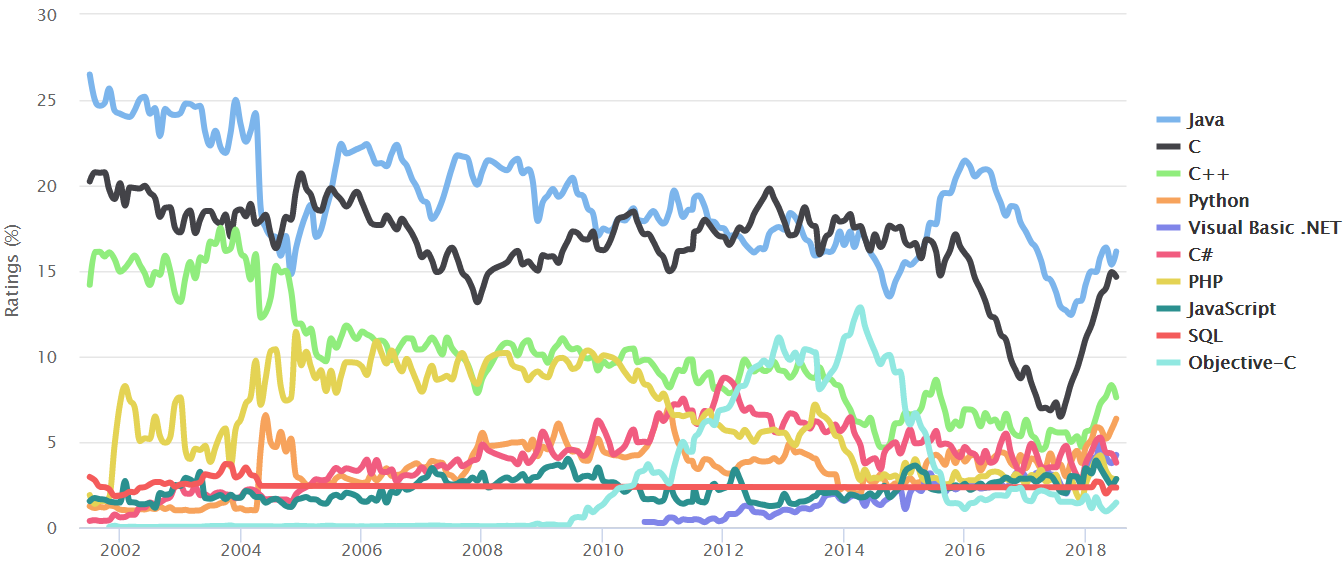
\includegraphics[width=\textwidth]{Immagini/Capitolo1/1_5-TrendTIOBE} 
\caption{TIOBE Programming Community index (\href{www.tiobe.com}{www.tiobe.com})}
\label{TIOBE}
\end{figure}

% --------------------------------------------------------------------------------------------------------------------------------------------
% SEZIONE 3
% --------------------------------------------------------------------------------------------------------------------------------------------
\section{Java choice}
\label{sec1.3}

The choice of Java as the programming language was driven by several considerations. These include the following:
\begin{itemize}
\item the language should be widely supported; this to avoid the case of many valid aircraft design applications and libraries that became obsolete due to the aging of the programming language used to build them;
\item the language is object oriented;
\item the language should promote the use of open source libraries, especially for I/O tasks and for complex mathematical operations;
\item the language and the companion Integrated Development Environment (IDE) should provide a widely supported Graphical User Interface (GUI) framework and a GUI visual builder;
\item the language should support and promote modularity.
\end{itemize}

The Java programming language meets all these requirements; moreover it is backed by Oracle and by a huge community of developers so it is continuously updated. Also, advanced and free IDEs (such as Eclipse) allow programmers to streamline and simplify the development process; in particular, the Eclipse IDE has been chosen to develop JPAD.

Being Java a pure object oriented programming language, it greatly encourages and simplifies modularization. Each module (package) can be programmed quite independently so that it is relatively easy to divide the work among several programmers. This is essential since the amount of classes and calculations needed to abstract, manage and analyse the entire aircraft is very large (presently the whole project counts more than 10 millions lines of code). For such a reason the establishment of common practices and the adherence to fundamental principle of software development (\emph{Don’t Repeat Yourself}, \emph{Separation of Concerns}, \emph{Agile software development}) are equally important.
% !TeX program = PdfLaTeX
% !TeX root = ../Main.tex

\chapter{Theoretical background}
\label{ch:ch2} %serve per citare il capitolo in un'altra sezione

Takeoff speeds are a safety key element for takeoff, and enable pilot situational
awareness and decision-making in this very dynamic situation. The use of erroneous
takeoff speeds can lead to tail strikes, high-speed rejected takeoff or initial climb with
degraded performance. 

% --------------------------------------------------------------------------------------------------------------------------------------------
% 								SEZIONE 1
% --------------------------------------------------------------------------------------------------------------------------------------------

\section{Take off speeds}
In this section a brief introduction to takeoff speeds will be provided \cite{Airbus:Flight:Notes}. \\
In aviation, these speeds are standard terms used to define airspeeds important or useful to the operation of all aircraft. They are derived from data obtained by aircraft designers and manufacturers during flight testing and verified in most countries by government flight inspectors during aircraft type-certification testing. Using them is considered a best practice to maximize aviation safety, aircraft performance or both. Takeoff speeds are calculated prior to a take off in accordance with aircraft weight, environmental factors etc.

\begin{figure}[htbp]
	\centering
	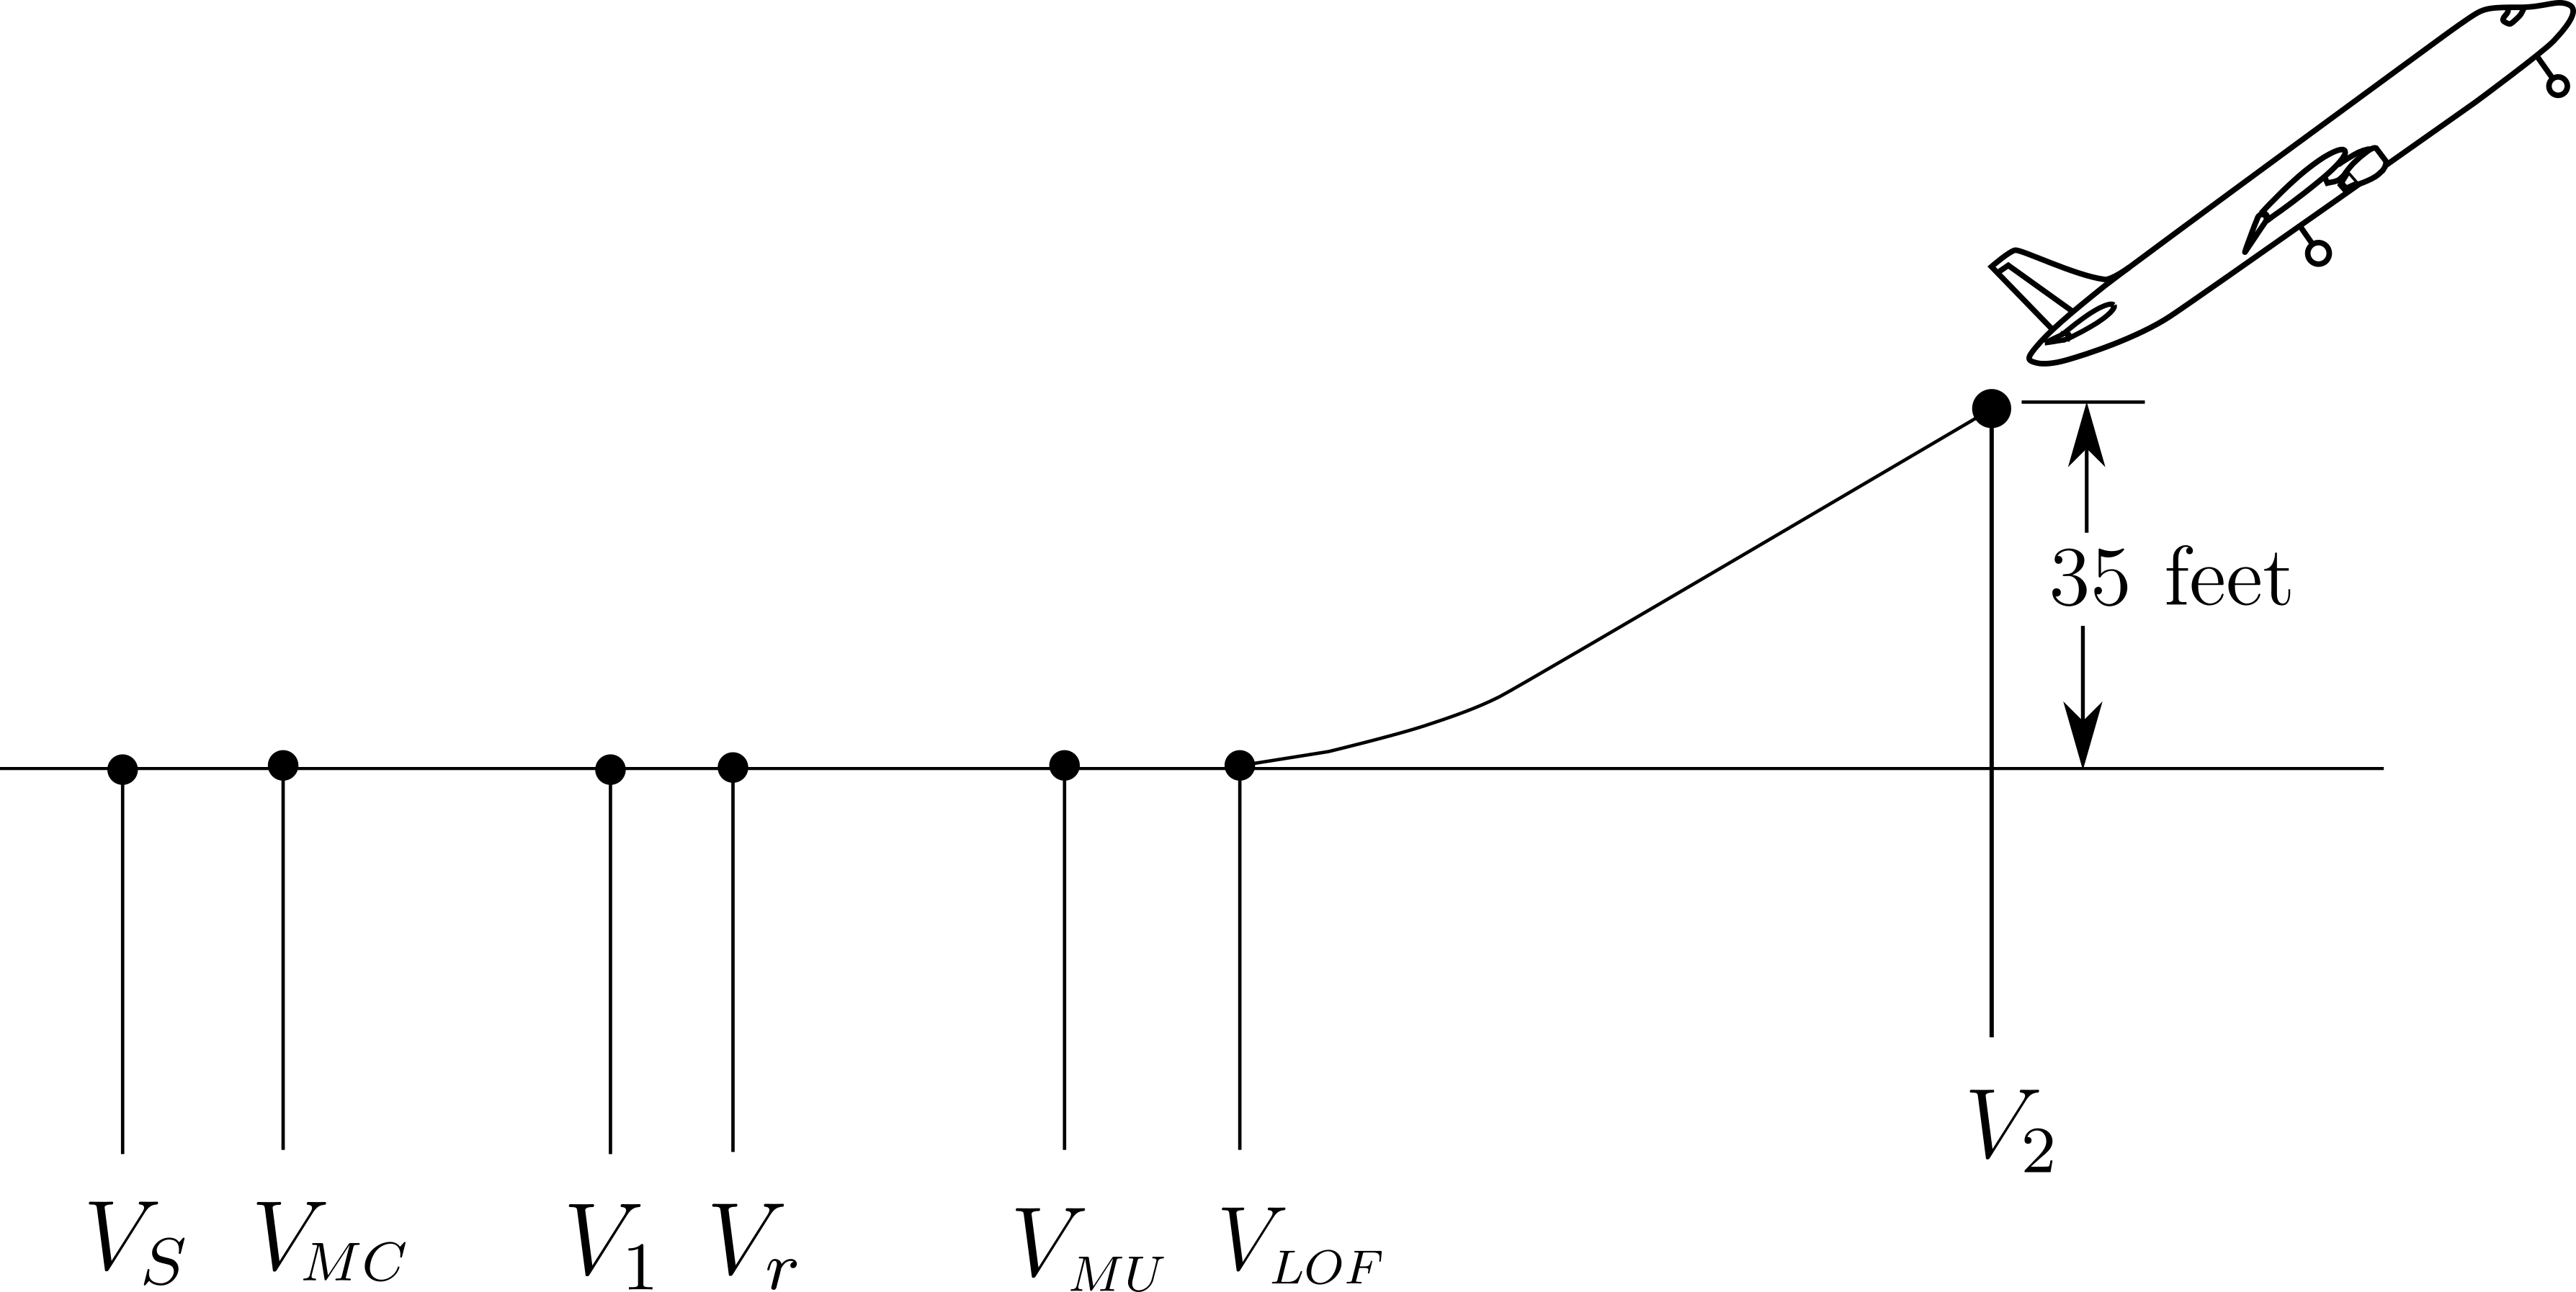
\includegraphics[height=7cm, keepaspectratio ]{Immagini/Capitolo2/takeoffSpeeds} 
	\caption{Takeoff speeds} % didascalia
	\label{fig:figura2_4} % etichetta per citarla nel testo
\end{figure}

\subsubsection{Velocity of stall $V_{S}$}
Aircraft stall speed during take off run.

\subsubsection{Velocity of Minimum Control $V_{MC}$}
During the takeoff roll, it is of utmost importance to know the minimum speed at which
the aircraft will remain controllable, in the event of an engine failure on ground. This is
because, in such a case, and if the takeoff is continued, only the rudder will be able to
counteract the yaw moment that is generated by asymmetric engine(s) thrust.
According to current regulations, the minimum speed at which an aircraft is defined to be “controllable”
(lateral excursion lower than 30 feet) after an engine failure on ground, is referred to
as $V_{MC}$ (Velocity of Minimum Control on Ground). 

\subsubsection{Decision Speed $V_1$}
$V_1$ is the maximum speed at which a rejected takeoff can be initiated, in the event of an
emergency. $V_1$ is also the minimum speed at which a pilot can continue a takeoff after an engine
failure.
If an engine failure is detected after $V_1$, the takeoff must be continued. This implies that
the aircraft must be controllable on ground. Therefore, V1 is always greater than $V_{MC}$.

\subsubsection{Rotation speed $V_r$}
Speed at which planes with a tricycle trolley lift the front wheel off the ground during take off.
 
\subsubsection{Velocity of Minimum Unstick $V_{MU}$}
 $V_{MU}$ is achieved by pitching the aircraft up to the maximum (tail on the runway, for
aircraft that are are geometrically-limited) during the takeoff roll (Refer to Figure~\ref{fig:figura2_1}). The speed at which the aircraft first lifts off is  $V_{MU}$. Therefore, lift-off is not
possible prior to  $V_{MU}$. 

\begin{figure}[htbp]
	\centering
	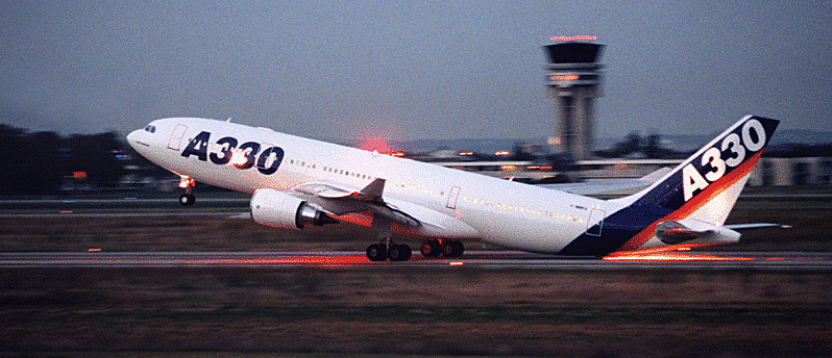
\includegraphics[height=6cm, keepaspectratio ]{Immagini/Capitolo2/2_1-VMUFlightTestOnAnA330} 
	\caption{$V_{MU}$ Flight Test on an Airbus A330} % didascalia
	\label{fig:figura2_1} % etichetta per citarla nel testo
\end{figure}

\subsubsection{Lift-off speed $V_{LOF}$}
Effective take off speed. It is assessed by adding a 10\% to the Minimum unstick speed with all the operating engines or a 5\% with an inoperative engine.

\subsubsection{Takeoff safety speed $V_2$}
$V_2$ is the speed at which the aircraft may safely be climbed with one engine inoperative. This speed is nicknamed a “take off safety speed”; it is the speed an aircraft with one engine inoperative must be able to attain in order to leave the runway and get 35 feet off the ground at the end of the runway, maintaining a 200 ft/min climb thereafter. This is the lowest speed at which the aircraft complies with the handling criteria associated with a climb after a take off, followed by the failure of an engine.

% --------------------------------------------------------------------------------------------------------------------------------------------
% 								SEZIONE 2	
% --------------------------------------------------------------------------------------------------------------------------------------------

\section{Ground effect}
Due to the fact that during the takeoff the aircraft is on the ground, in order to asses $V_{MU}$,  it is important to consider the ground effect. This generally become measurable at a height above the ground of one wing-span and increase in magnitude as the height above the ground decreases. Both theoretical and
experimental investigations indicate that ground proximity produces an increase in the lift-curve
slope, a decrease in drag, and a reduction of nose-up pitching moment for most aircraft planforms in
the clean configuration. However, high-lift configurations deviate from this trend in that the ground
effect tends to reduce the lift-curve slope \cite{Datcom}.\\

The majority of the theoretical approaches analyzing ground effects employ an image-vortex theory
to represent the ground plane. The salient aspects of this theory are discussed below.\\

Away from the ground plane, the downwash of the two trailing vortices contributes to the wing
drag die to lift by rotating the force vector rearward.\\
However, near the ground plane, the trailing vortices of the image vortex system have an upwash component.\\

This upwash velocity component reduces the downward rotation of the flow direction caused by the wing trailing vortices, thus decreasing the wing drag due to lift.\\

The ground effects on lift are determined somewhat by the planform of the configuration. For
low-aspect-ratio delta configurations, the general trend is a constant increase in $C_L$ due to ground
effect, as shown in figure~\ref{fig:figura2_2}.
However, transport-type configurations show quite a different trend, as presented in figure~\ref{fig:figura2_3}.\\
This trend is dependent upon tie type of high-lift system employed.

\begin{figure}[htbp]
	\centering
	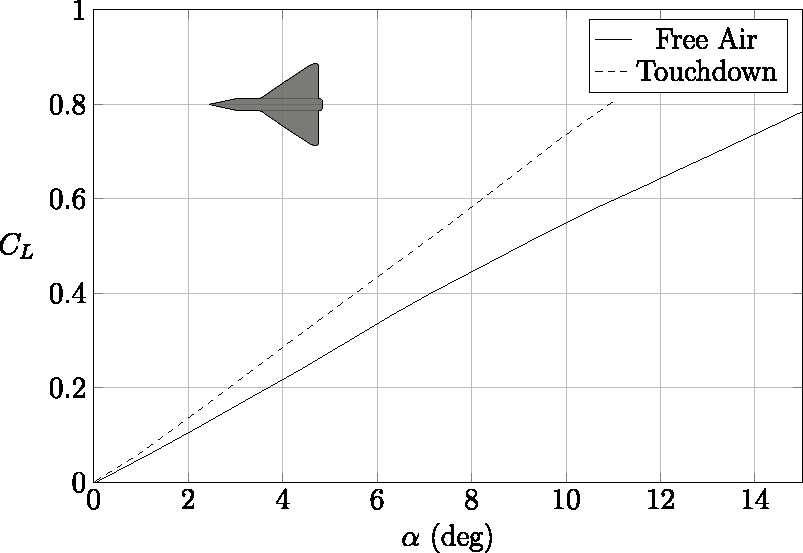
\includegraphics[height=10cm, keepaspectratio ]{Immagini/Capitolo2/2_2-GroundEffectDeltaConf} 
	\caption{Ground effect on 55°  delta configuration} % didascalia
	\label{fig:figura2_2} % etichetta per citarla nel testo
\end{figure}

\begin{figure}[htbp]
	\centering
	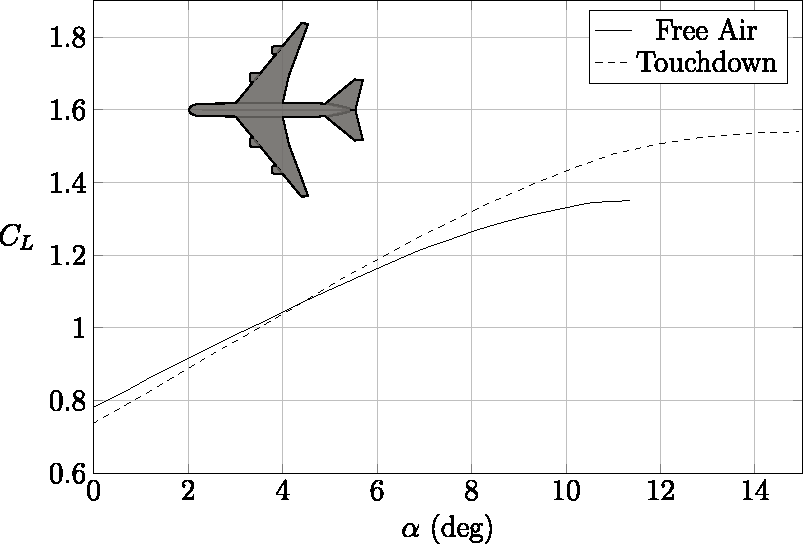
\includegraphics[height=10cm, keepaspectratio ]{Immagini/Capitolo2/2_3-GroundEffectJetTranspConf} 
	\caption{Ground effect on a jet transport configuration} % didascalia
	\label{fig:figura2_3} % etichetta per citarla nel testo
\end{figure}

\section{Datcom methods}
\label{sec:sec3}
For most vehicles, calculating the change in lift due to ground effects consists of evaluating two
components:
 \begin{enumerate}
 \item the change in wing-body lift;
 \item the change in tail-body lift due to the effects of downwash.
 \end{enumerate}
 
The change in tail-body lift due to the presence of the ground is generally small in comparison to
the downwash effects and is neglected in the Datcom methods.\\
Both of the Datcom methods presented require the user to construct wing-body and tail-body lift
curves in ground effect based on their corresponding free-air lift curves. Equations are given that
calculate the change in angie of attack due to ground effect at a constant lift coefficient. The
ground-effect lift curves are then constructed by shifting the free-air lift curves at every $C_L$ by the
corresponding increment in angle of attack due to ground effect at constant lift coefficients.

\begin{figure}[htbp]
	\centering
	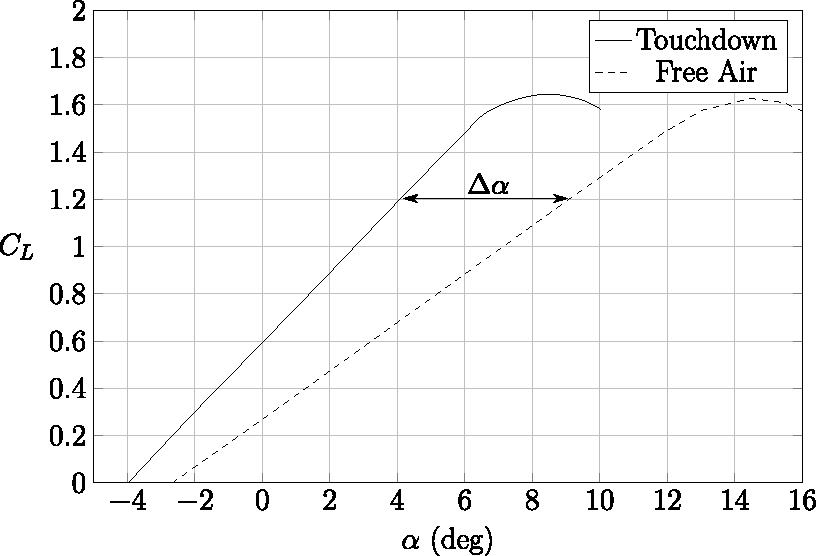
\includegraphics[height=10cm, keepaspectratio ]{Immagini/Capitolo2/disegno} 
	\caption{Ground effect on a jet transport configuration} % didascalia
	\label{fig:figura2_3_1} % etichetta per citarla nel testo
\end{figure}

\subsubsection{Method I}
This method estimates the ground effects on lift in the linear-lift range for a subsonic transport
configuration. It includes the effects of taper ratio, sweep-back, dihedral, and flap deflection, while neglecting the effects of
wing thickness since they are generally small. The wing-flap effects are valid only for split and slotted flaps as they are accounted for by empirical curves. \\
The change in wing-body angle of attack at a constant lift coefficient due to ground effect with
respect to the out-of-ground-effect lift curve is given by:

\begin{equation}
\begin{split}
\left(\Delta \alpha\right)_G=&-\left[\frac{9.12}{\AR}+7.16\left(\frac{c_r}{b}\right)\right]\left( C_{L_f} \right)_{WB}x \ +\\
&-\frac{\AR}{2\left( C_{L_{\alpha}} \right)_{WB}}\left(\frac{c_r}{b}\right)\left(\frac{L}{L_0}-1\right)\left( C_{L_f} \right)_{WB}r \ + \\ &-\frac{\left(\delta_f /50\right)^2}{\left( C_{L_{\alpha}} \right)_{WB}}\Delta \left(\Delta C_L \right)_{flap} \ \text{(per  deg)}
\label{eq:equazione2_1} % etichetta per citarla nel testo
\end{split}
\end{equation}
\\ \\ \\ \\  where\\ \\ \\
\begin{tabulary}{1\textwidth}{L L}
\begin{minipage}[T]{6cm}$\Delta \left(\Delta C_L \right)_{flap}$  \end{minipage}& is an empirical factor to account for the effect of flaps and is obtained from~\vref{fig:figura2_4} as a function of the height of the quarter-chord point of the wing root chord above the ground,\\ \\
\AR & is the wing aspect ratio, \\ \\
$\dfrac{c_r}{b}$ & is the ratio of wing root chord to wing span, \\ \\
$\left( C_{L_f} \right)_{WB} $ & is the wing-body lift coefficient including flap effects, out of ground effect, \\ \\
$x$ & accounts for the effects on lift due to the image trailing vortex and is obtained
from~\vref{fig:figura2_6} as a function of wing geometry and the wing height above
the ground, \\ \\
$\dfrac{L}{L_0}-1 $ & accounts for the effects on lift due to the image bound vortex and is obtained from~\vref{fig:figura2_8} as a function of wing geometry, lift coefficient, and the height of the quarter-chord point of the wing root chord above the ground. \\ \\
$\left( C_{L_{\alpha}} \right)_{WB} $  & is the wing body lift-curve slope, per degree, out of  ground effect \\ \\
$r$ & accounts for the effect of finite span and is obtained from~\vref{fig:figura2_9} as a function of wing height above the ground, \\ \\
\end{tabulary}

The first term in Equation~\ref{eq:equazione2_1} accounts for the effects of he trailing vortex, the second term for the effects of the trailing vortex, the second term for the effects of the bound vortex, and the third term for wing-flap effects. The method does not account for the effects of wing-leading-edge devices.\\
\begin{figure}[H]
	\centering
	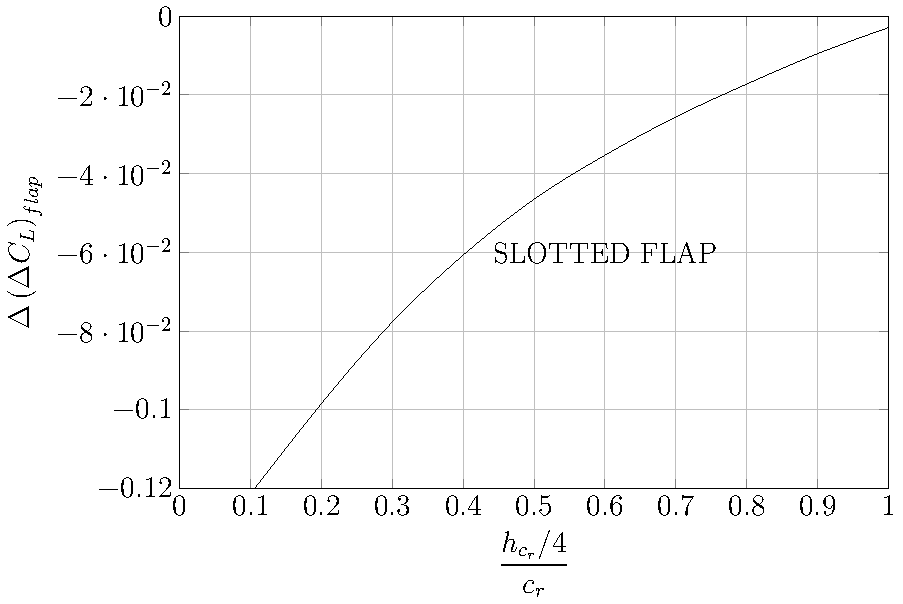
\includegraphics[height=7.3cm, keepaspectratio ]{Immagini/Capitolo2/2_4-Delta_alpha_CL_Ground_Effect_DeltaDelta_CL_flap_vs_h_cr_4_cr} 
	\caption{Effect of flap deflection on the ground influence on lift} % didascalia
	\label{fig:figura2_4} % etichetta per citarla nel testo
\end{figure}

\begin{figure}[H]
	\centering
	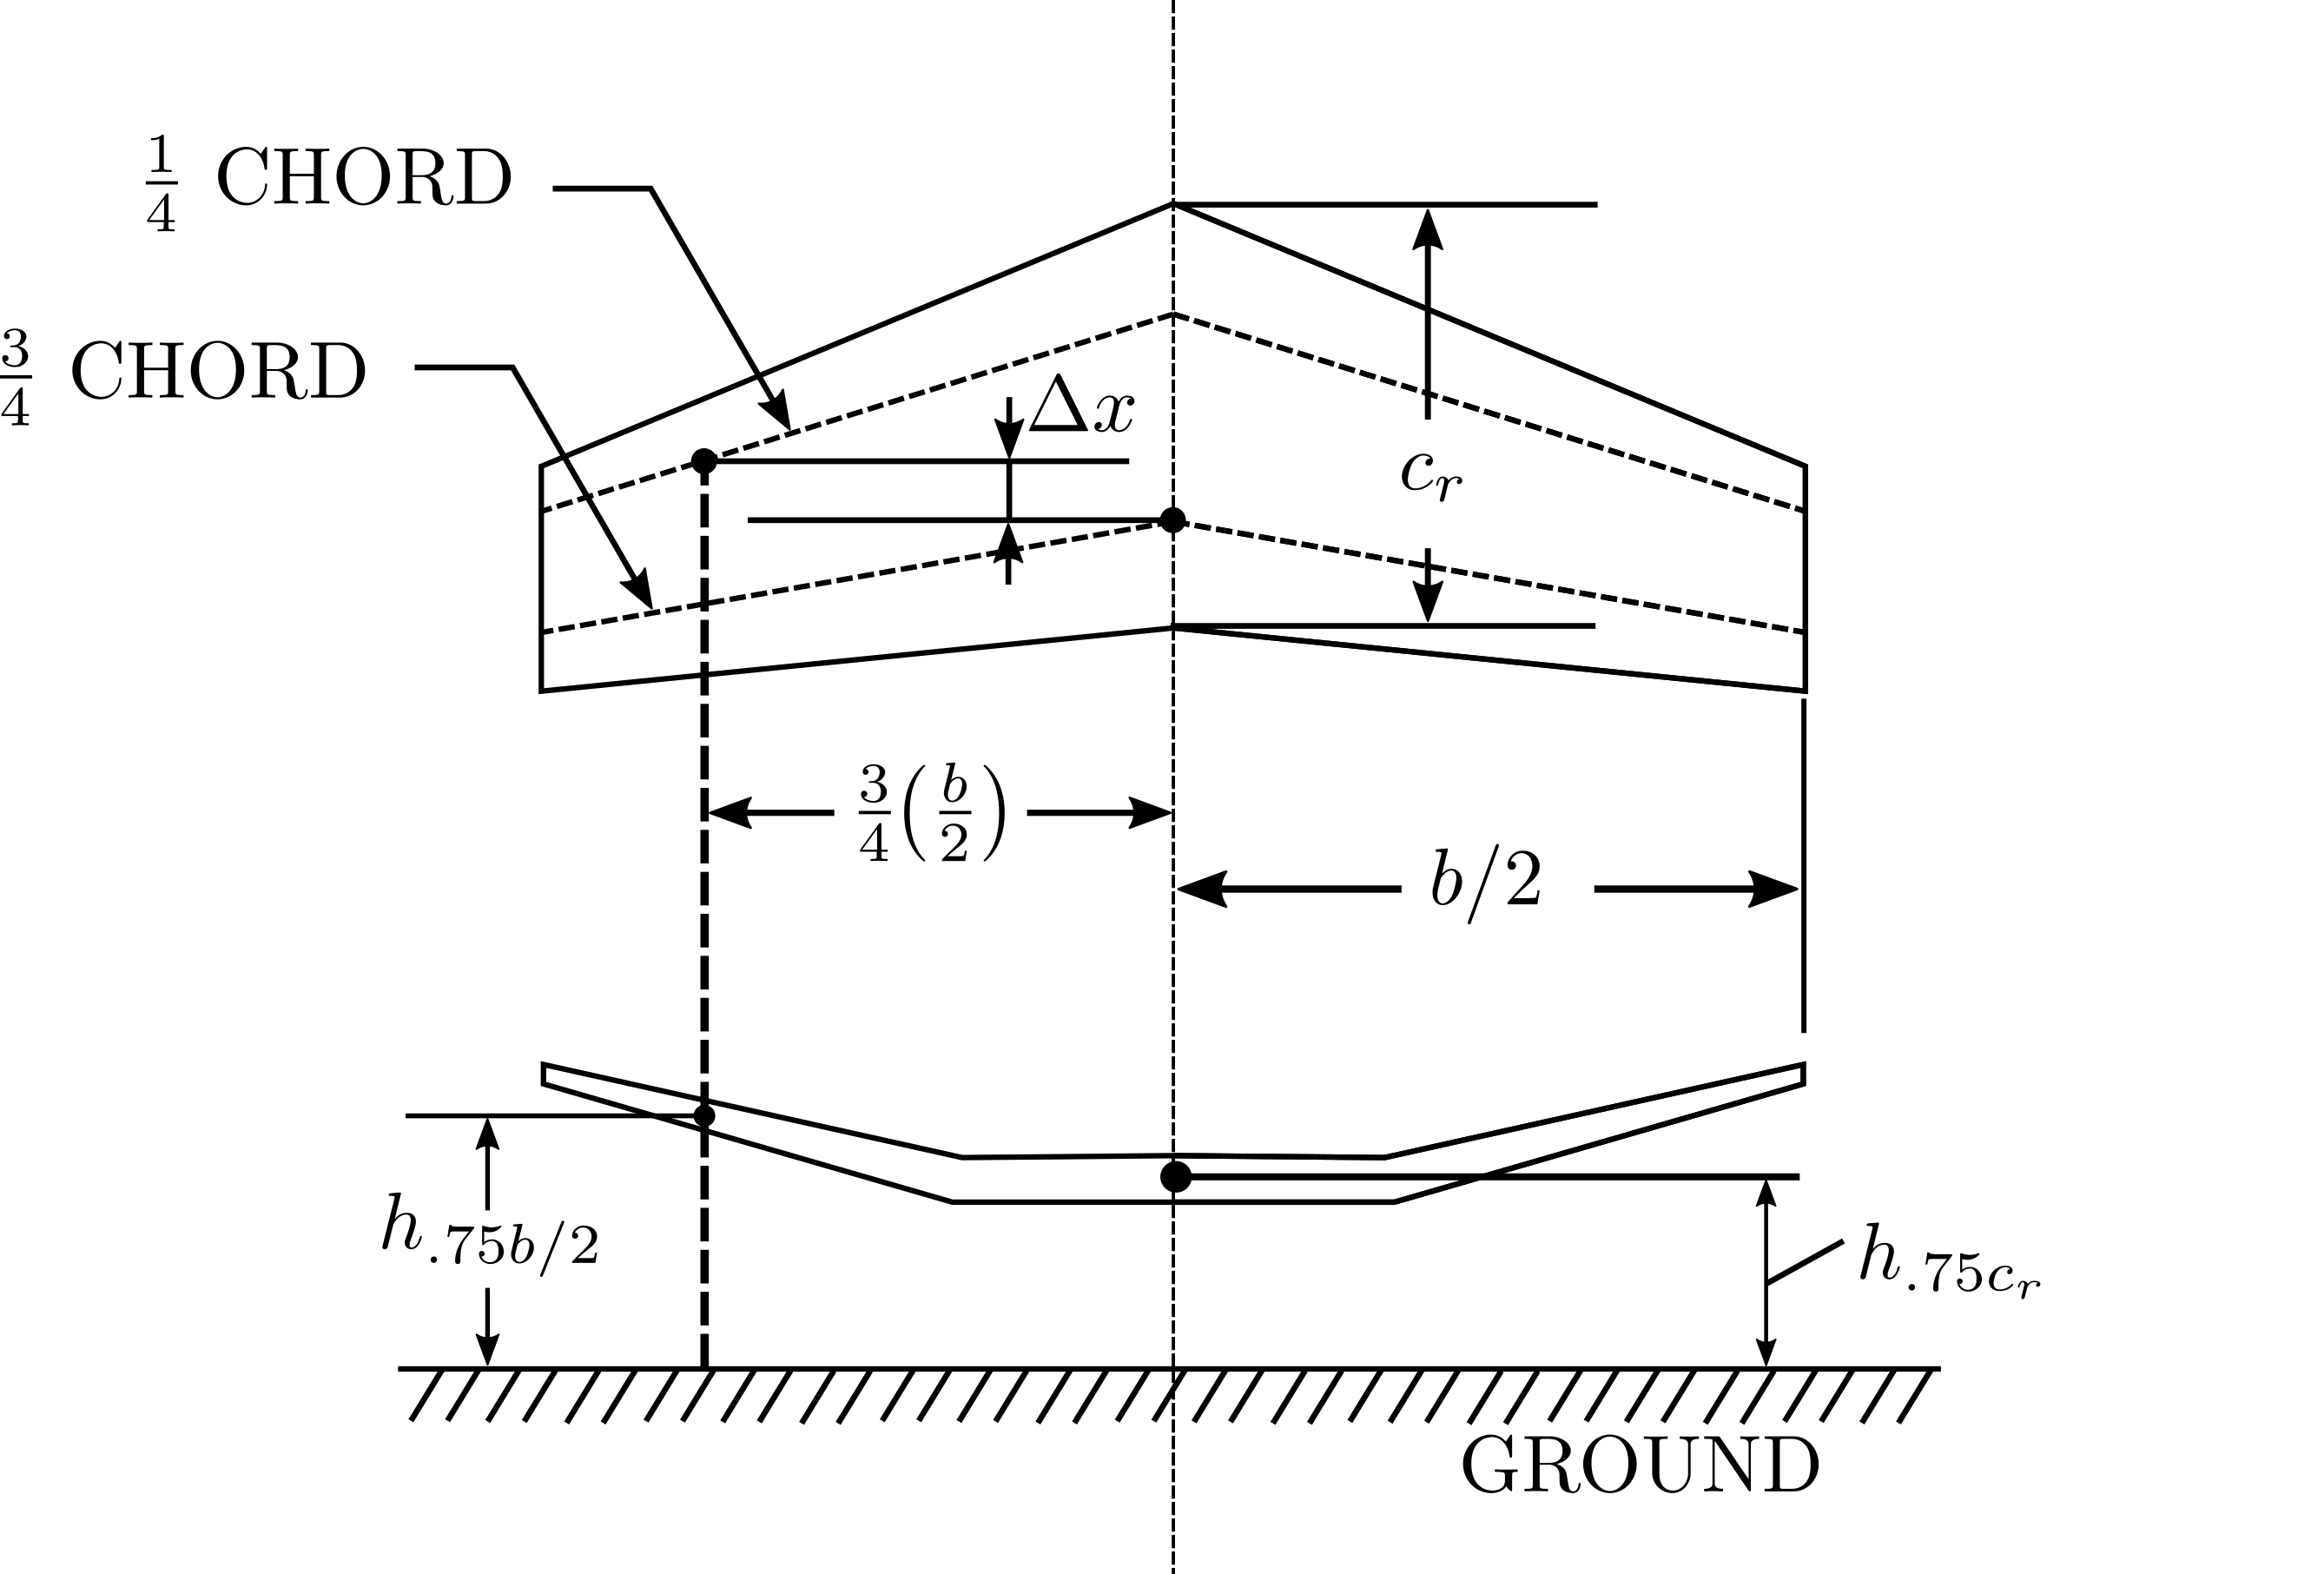
\includegraphics[height=9cm, keepaspectratio ]{Immagini/Capitolo2/disegno-1} 
	\caption{Description of geometric parameters} % didascalia
	\label{fig:figura2_5} % etichetta per citarla nel testo
\end{figure}

where
\[\frac{h}{b/2}=\frac{0.5\left(h_{.75b/2}+h_{.75c_r}\right)}{b/2}\]

\begin{figure}[H]
	\centering
	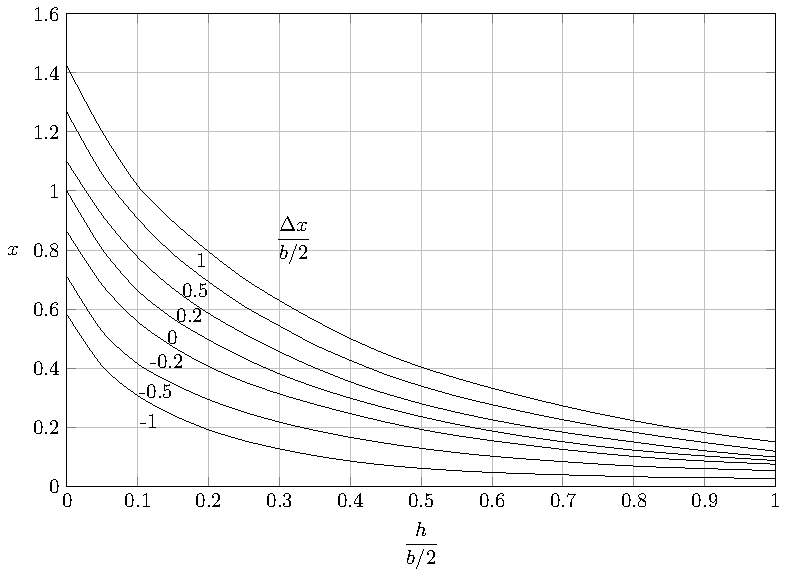
\includegraphics[height=9.5cm, keepaspectratio ]{Immagini/Capitolo2/2_6-(Delta_alpha_CL_Ground_Effect)_x_vs_2hfracb_Deltax} 
	\caption{Parameter accounting for ground effect on lift due to trailing vortices} % didascalia
	\label{fig:figura2_6} % etichetta per citarla nel testo
\end{figure}


\begin{figure}[H]
	%\centering
	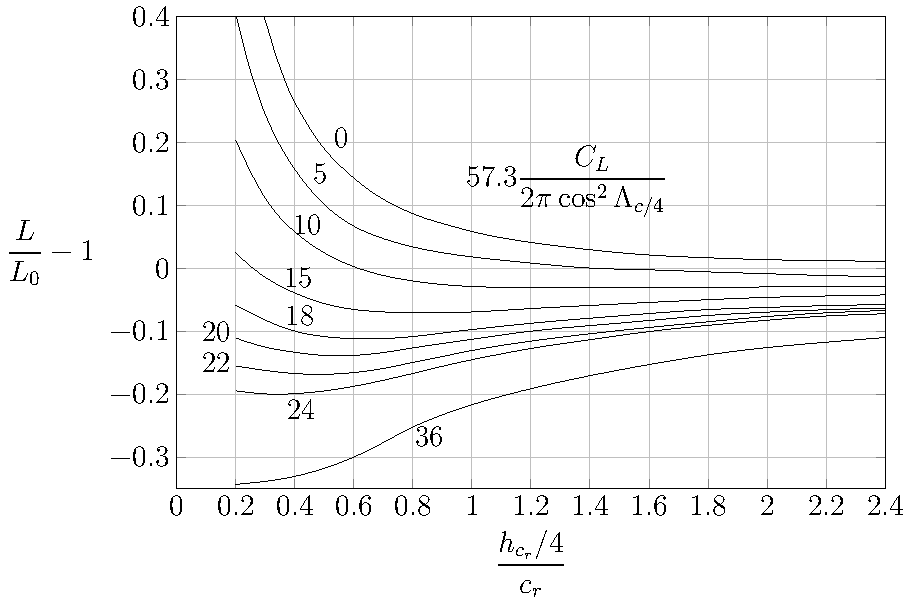
\includegraphics[height=8.5cm, keepaspectratio ]{Immagini/Capitolo2/2_8-Delta_alpha_CL_Ground_Effect_L_L0_minus1_vs_h_cr_4_cr} 
	\caption{Parameter accounting for ground effect on lift due to bound vortices} % didascalia
	\label{fig:figura2_8} % etichetta per citarla nel testo
\end{figure}

\begin{figure}[H]
	\centering
	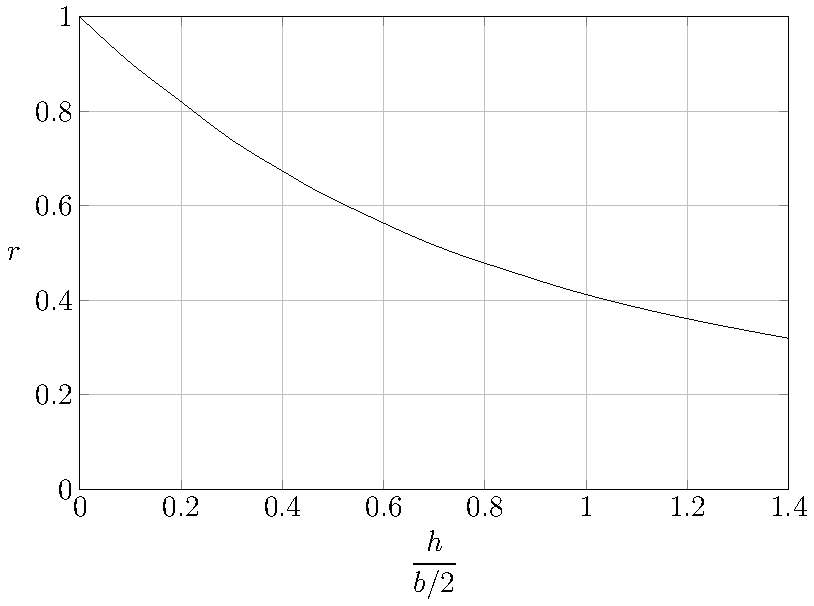
\includegraphics[height=8.5cm, keepaspectratio ]{Immagini/Capitolo2/2_9-Delta_alpha_G_r_vs_2hfracb} 
	\caption{Factor accounting for finite span in ground effect} % didascalia
	\label{fig:figura2_9} % etichetta per citarla nel testo
\end{figure}

In the linear-lift region, the change in downwash (a decrease) on this tail-body due to ground effects
is derived theoretically by representing the ground plane as an image-vortex system.\\
The change (a decrease) in tail-body downwash due to ground effects in the linear-lift range is given by:

\begin{equation}
\left(\Delta \varepsilon \right)_G=\varepsilon \left[\frac{b_{eff}^2+4\left(H_H+H\right)^2}{b_{eff}^2+4\left(H_H-H\right)^2}\right]
\label{eq:equazione2_2} % etichetta per citarla nel testo
\end{equation}
where \\ \\

\begin{tabulary}{1\textwidth}{L L}
\begin{minipage}[T]{3cm}$\left(\Delta \varepsilon \right)_G$  \end{minipage}& is the difference between the downwash in free air and the downwash in
ground effect,\\ \\
$\varepsilon$ & is the downwash out of ground effect, \\ \\
$H$ & is the height of $\frac{\overline c}{4}$ of the wing above the ground, \\ \\
$H_H$ & is the height of $\frac{\overline c}{4}$ of the horizontal tail above the ground.\\ \\
$b_{eff}$ & is the effective wing span defined as\\ \\
\end{tabulary}

\begin{equation}
b_{eff}=\frac{ C_{L_{WB}} +\Delta C_{L_f} }{\dfrac{ C_{L_{WB}} }{b'_W}+ \dfrac {\Delta C_{L_f} }{b'_f}}
\label{eq:equazione2_2_1} % etichetta per citarla nel testo
\end{equation}
  \indent \indent \indent  where \\ \\

\begin{tabulary}{1\textwidth}{L L}
\begin{minipage}[T]{4cm}$\qquad \qquad  C_{L_{WB}}$  \end{minipage}&  is the wing-body lift coefficient, flaps retracted, out of ground effect,\\ \\
$\qquad \qquad  \Delta C_{L_f}$ & is the change in lift coefficient due to flaps, out of ground effect. \\ \\
\end{tabulary}

\begin{equation}
b'_W=\left(\frac{b'_W}{b}\right)b
\label{eq:equazione2_3_1} % etichetta per citarla nel testo
\end{equation}

\begin{equation}
b'_W=\left(\frac{b'_f}{b'_W}\right)\left(\frac{b'_W}{b}\right)b
\label{eq:equazione2_3_2} % etichetta per citarla nel testo
\end{equation}
 \indent \indent \indent The ratio $\dfrac{b'_W}{b}$ is given in~\vref{figura2_10} as a function of taper \indent \indent \indent ratio and aspect ratio, and $\dfrac{b'_f}{b'_W}$ is given in~\vref{fig:figura2_11} as   \indent \indent \indent a function of the  ratio  of flap span to wing span.\\
 
The horizontal-tail lift curve in ground effect is constructed by shifting the free-air lift curve at
every $C_L$ by the corresponding \(-\left(\Delta \varepsilon \right)_G\), i.e.,
\begin{equation}
\left(\Delta \alpha_H \right)_G=-\left(\Delta \varepsilon \right)_G
\label{eq:equazione2_3} % etichetta per citarla nel testo
\end{equation}

 \begin{figure}[H]
	%\centering
	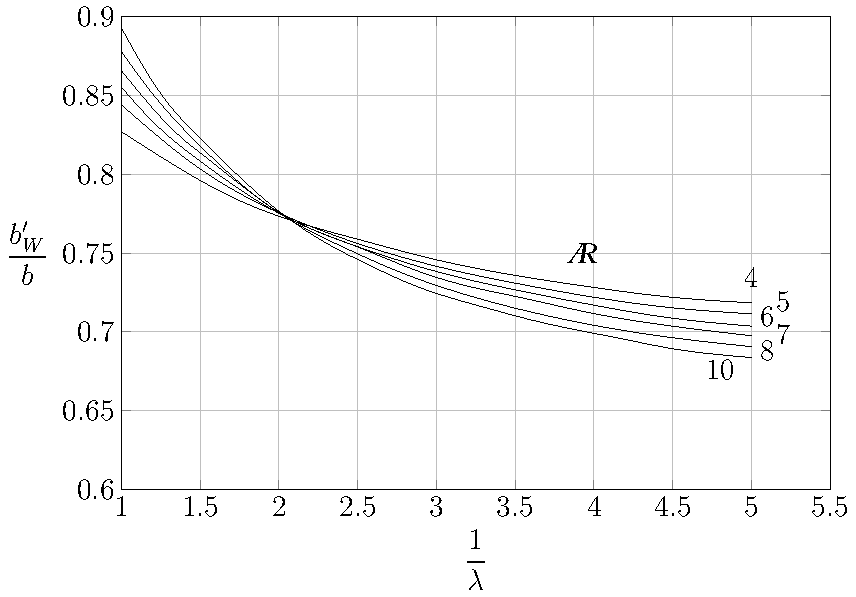
\includegraphics[height=10.5cm, keepaspectratio ]{Immagini/Capitolo2/2_10-bapexwfracb} 
	\caption{Effective wing span in the presence of the ground} % didascalia
	\label{figura2_10} % etichetta per citarla nel testo
\end{figure}

\begin{figure}[H]
	\centering
	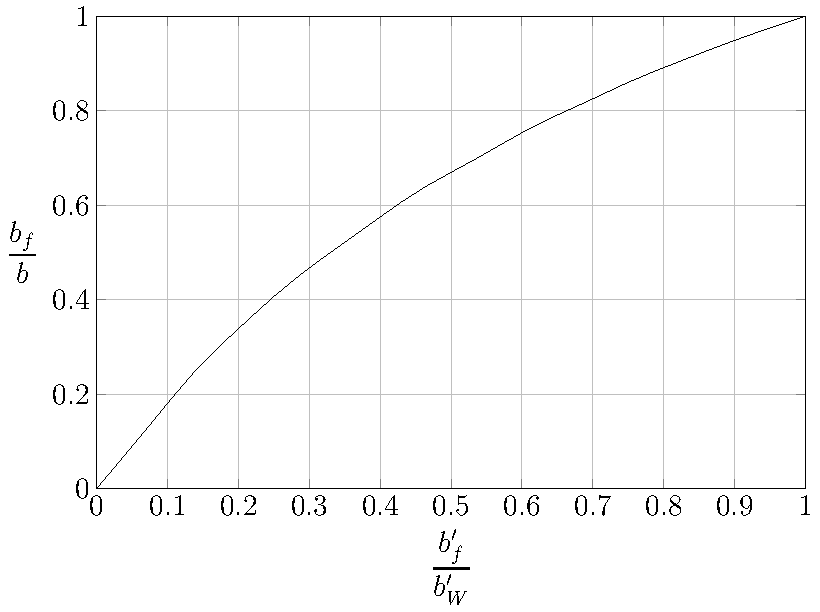
\includegraphics[height=10.5cm, keepaspectratio ]{Immagini/Capitolo2/2_11-bapexffracbapexw} 
	\caption{Effective flap span in the presence of the ground} % didascalia
	\label{fig:figura2_11} % etichetta per citarla nel testo
\end{figure}

\subsubsection{Method II}
This method estimates the ground effects on wing-body lift in the linear-lift range for all
configurations not included in Method I.
The change in wing-body angle of attack due to ground
effects with respect to the out-of-ground-effect lift curve is given by:

\begin{equation}
\left(\Delta \alpha\right)_G=-18.4\frac{\left( C_{L_f} \right)_{WB}\sigma}{\AR}+rT\frac{\left( C_{L_f} \right)_{WB}^2}{57.3\left( C_{L_{\alpha}} \right)_{WB}}-rB+K\left(\frac{t}{c}\right)_{max} \ \text{(per  deg)}
\label{eq:equazione2_4} % etichetta per citarla nel testo
\end{equation}
\\ \\   where\\ \\ \\
\begin{tabulary}{1\textwidth}{L L}
\begin{minipage}[T]{6cm}$\sigma$  \end{minipage}& is Prandtl's interference coefficient from multiplane theory and is obtained from~\vref{fig:figura2_12} as a function of wing height above the ground,\\ \\
$r$ & accounts for the effect of finite span and is obtained from~\vref{fig:figura2_9} as a function of wing height above the ground, \\ \\
$T$ & accounts for the reduction of the longitudinal velocity and is obtained from~\vref{fig:figura2_13} as a function of wing height above the ground, \\ \\
$B$ &accounts for the change in circulation and is obtained from~\vref{fig:figura2_14} as a function of wing height above the ground, \\ \\
$K$ & accounts for the effective wing thickness and is obtained from~\vref{fig:figura2_15} as a function of wing height above the ground, \\ \\
$\left(C_{L_{\alpha}} \right)_{WB}$ & is the wing-body lift-curve slope, per degree, out of ground effect, \\ \\
$\left(\dfrac{t}{c}\right)_{max}$  & is the ratio of maximum wing thickness to wing chord, \\ \\
$\left( C_{L_f} \right)_{WB}$ & is the wing-body lift coefficient including flap effects, out of ground effect. \\ \\
\end{tabulary}

\begin{figure}[H]
	\centering
	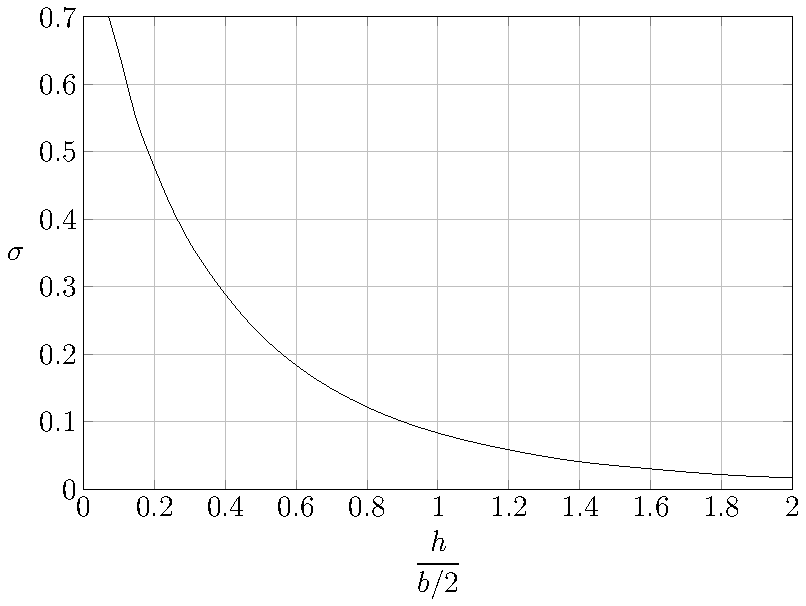
\includegraphics[height=10.5cm, keepaspectratio ]{Immagini/Capitolo2/2_12-(Delta_alpha_G)_sigma_vs_2hfracb} 
	\caption{Prandtl's interference coefficient - indicative of variation in induced vertical velocity with ground effect} % didascalia
	\label{fig:figura2_12} % etichetta per citarla nel testo
\end{figure}

\begin{figure}[H]
	\centering
	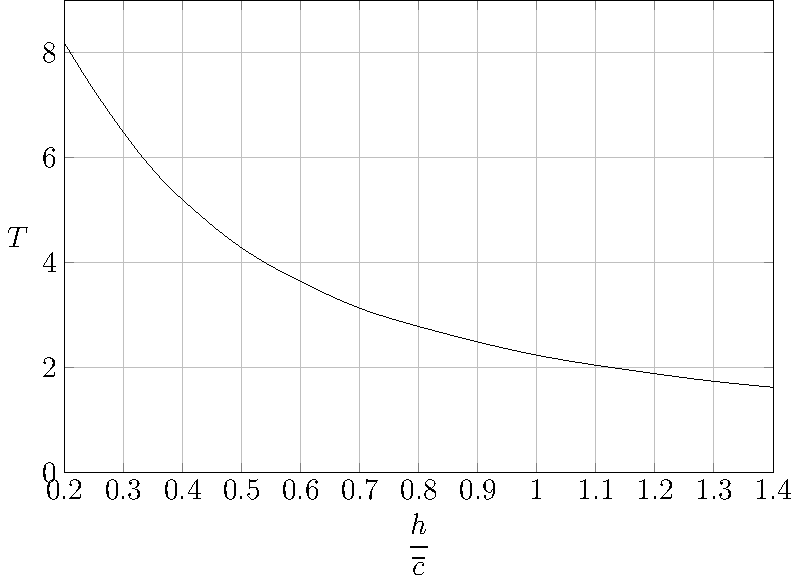
\includegraphics[height=10.5cm, keepaspectratio ]{Immagini/Capitolo2/2_13-(Delta_alpha_G)_T_vs_h_frac_overline_c} 
	\caption{Parameter accounting for variation in longitudinal velocity with ground height} % didascalia
	\label{fig:figura2_13} % etichetta per citarla nel testo
\end{figure}

\begin{figure}[H]
	%\centering
	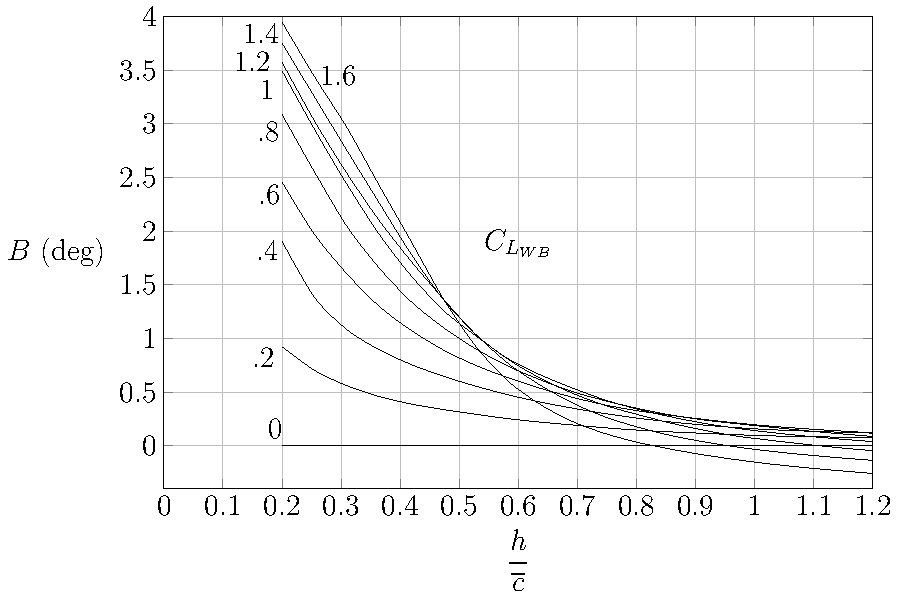
\includegraphics[height=9.5cm, keepaspectratio ]{Immagini/Capitolo2/2_14-(Delta_alpha_G)_B_vs_h_frac_overline_c_C_L_WB} 
	\caption{Parameter accounting for variation in circulation with lift and height above ground} % didascalia
	\label{fig:figura2_14} % etichetta per citarla nel testo
\end{figure}

\begin{figure}[H]
	\centering
	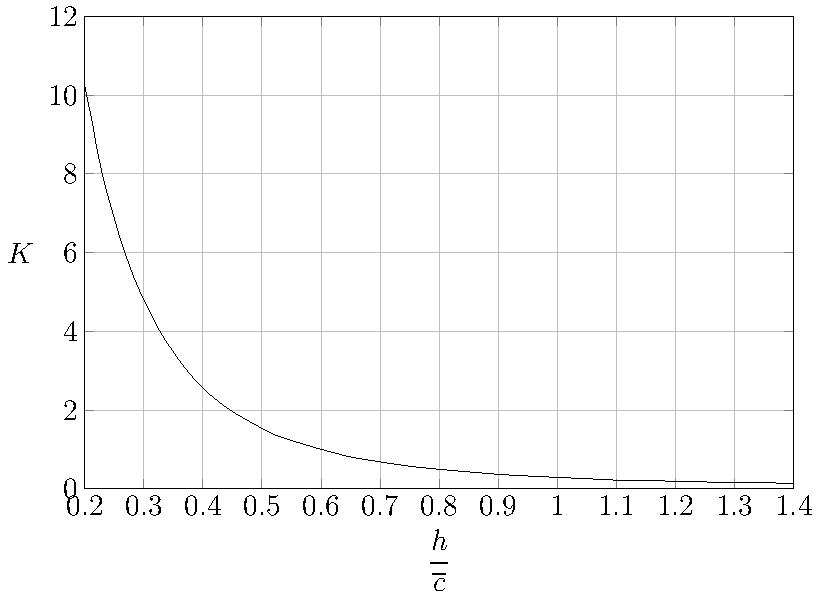
\includegraphics[height=10.5cm, keepaspectratio ]{Immagini/Capitolo2/2_15-Delta_alpha_G_K_vs_h_frac_c} 
	\caption{Parameter accounting for influence of wing thickness due to height above ground} % didascalia
	\label{fig:figura2_15} % etichetta per citarla nel testo
\end{figure}


% --------------------------------------------------------------------------------------------------------------------------------------------
% 								SEZIONE 3
% --------------------------------------------------------------------------------------------------------------------------------------------

\section{Assessment of minimum unstick speed}
The aircraft will be in the takeoff configuration at the maximum angle of attack allowed by the geometry, as shown in~\vref{fig:figura2_16}
\begin{figure}[H]
	\centering
	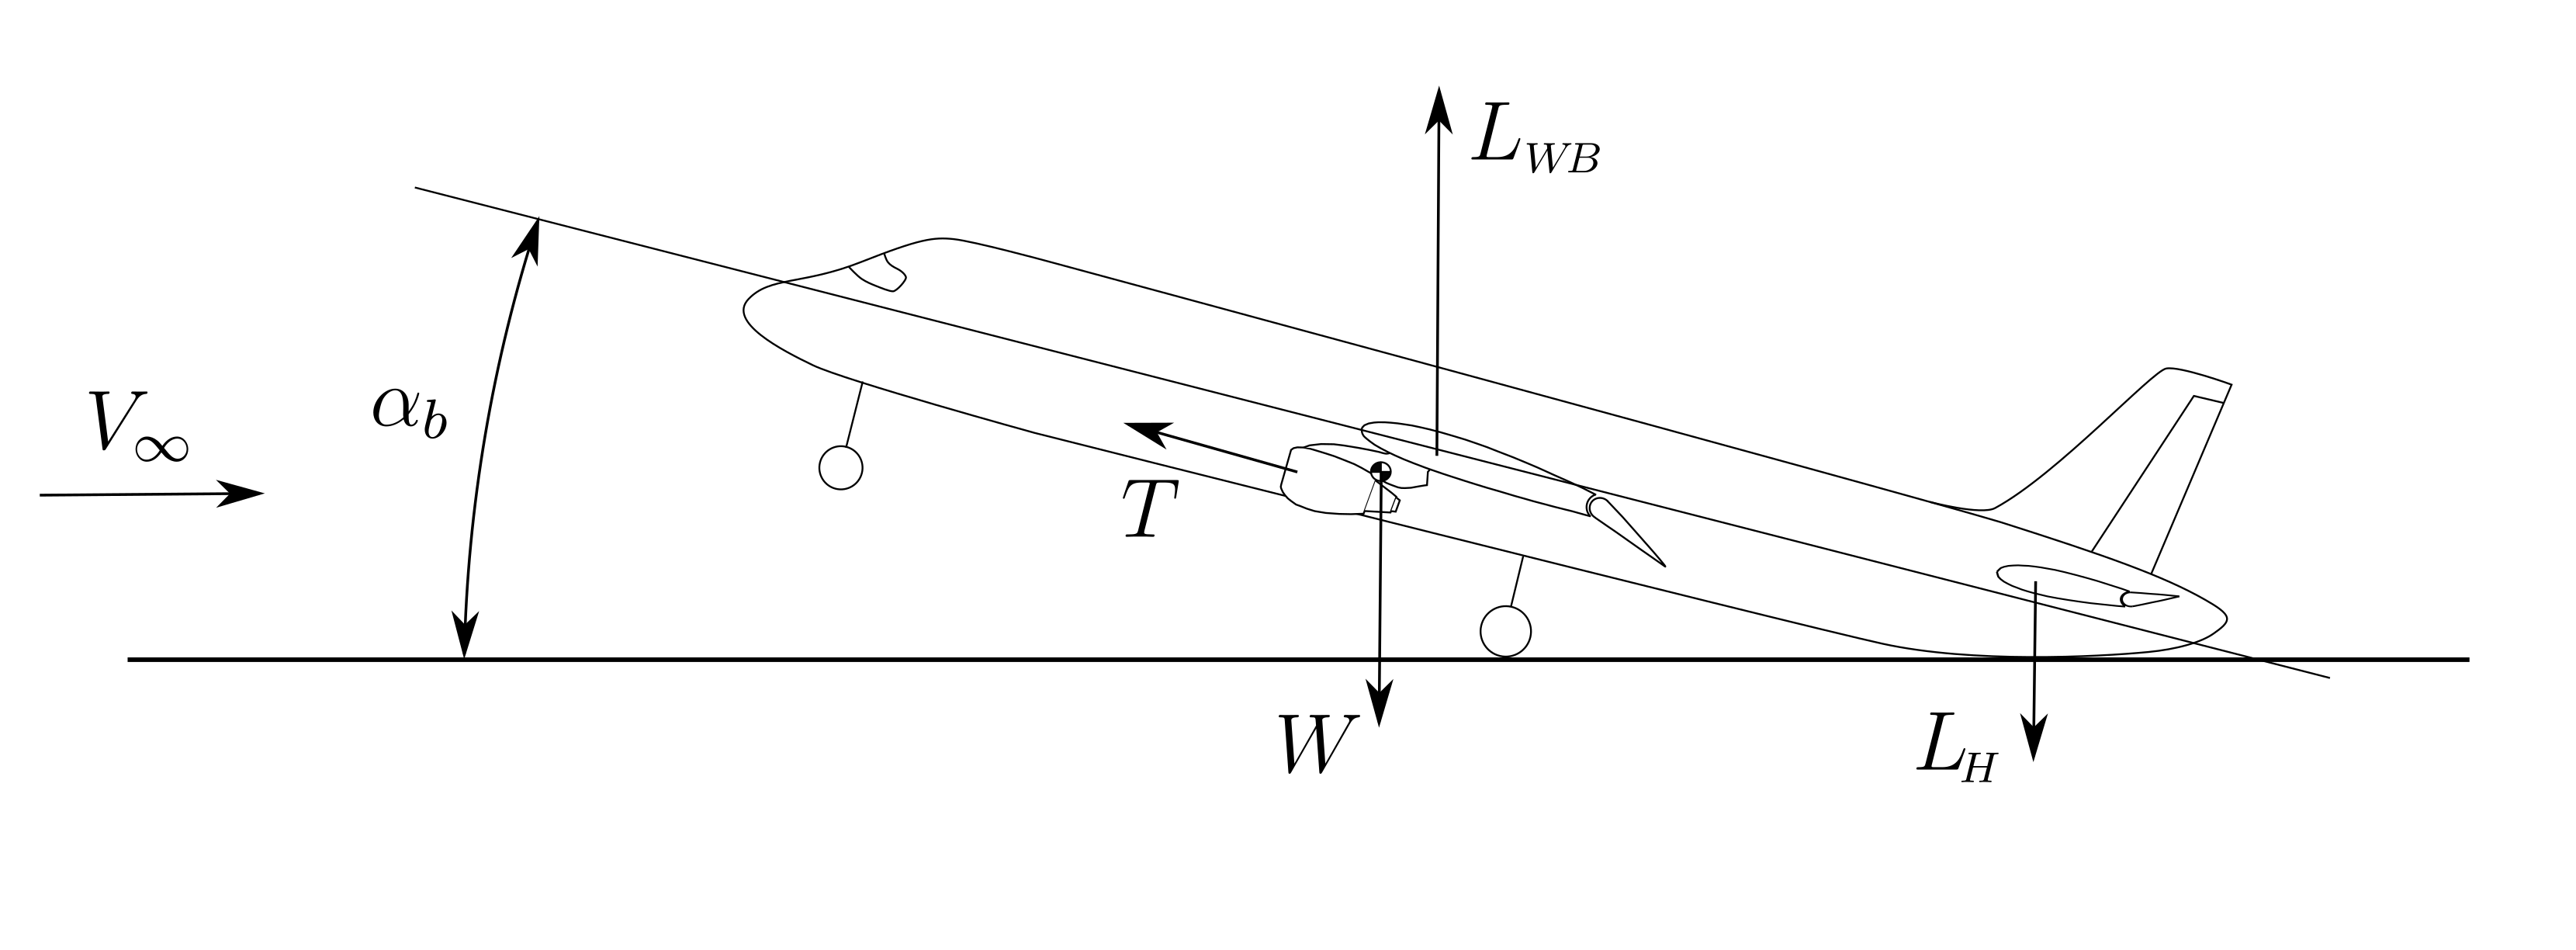
\includegraphics[height=5cm, keepaspectratio ]{Immagini/Capitolo2/2_16-aereoVmu} 
	\caption{Takeoff configuration for the assessment of VMU} % didascalia
	\label{fig:figura2_16} % etichetta per citarla nel testo
\end{figure}

Known the geometry of the fuselage can be calculated $\alpha_{W}$ and $\alpha_{H}$:

\[\alpha_{W}=\alpha_{b}+i_W\]
\[\alpha_{H}=\alpha_{b}-\varepsilon+i_H\]

The $V_{MU}$  is the speed at which the aircraft takes off in this configuration, i.e. the speed that makes the 
algebraic sum of lift (wing-body lift and horizontal tail lift) and thrust upwards component equals to the weight of the aircraft.\\
In formulas:

\begin{equation}
L_{TOT}=L_{WB}+L_H+T\sin \alpha_b=W
\label{eq:equazione2_5} % etichetta per citarla nel testo
\end{equation}
\begin{equation}
L_{TOT}=C_{L_{WB}}\frac{1}{2}\rho V_{\infty}^2S_W+C_{L_{H}}\frac{1}{2}\rho V_{\infty}^2 \eta S_H+T\sin \alpha_b=W
\label{eq:equazione2_6} % etichetta per citarla nel testo
\end{equation}
from which it is obtained:
\begin{equation}
V_{MU}=\sqrt{\frac{W-T\sin \alpha_b}{C_{L_{WB}}\frac{1}{2}\rho S_W+C{L_H}\frac{1}{2}\rho  \eta S_H}}
\label{eq:equazione2_6} % etichetta per citarla nel testo
\end{equation}
where $C_{L_{WB}}$ and $C_{L_H}$  are influenced by the ground effect. In particular there will be a new wing-body lift coefficient curve and new downwash angle as shown in section~\ref{sec:sec3}.

% !TeX program = PdfLaTeX
% !TeX root = ../Main.tex

\chapter{Results and analysis}
\label{ch3}

In this chapter is presented a case study performed on a regional turboprop of 130 pax, concerning aerodynamic characteristics, high lift devices and ground effect both on wing lift curve and on downwash angle.

\begin{figure}[H]
	\centering
	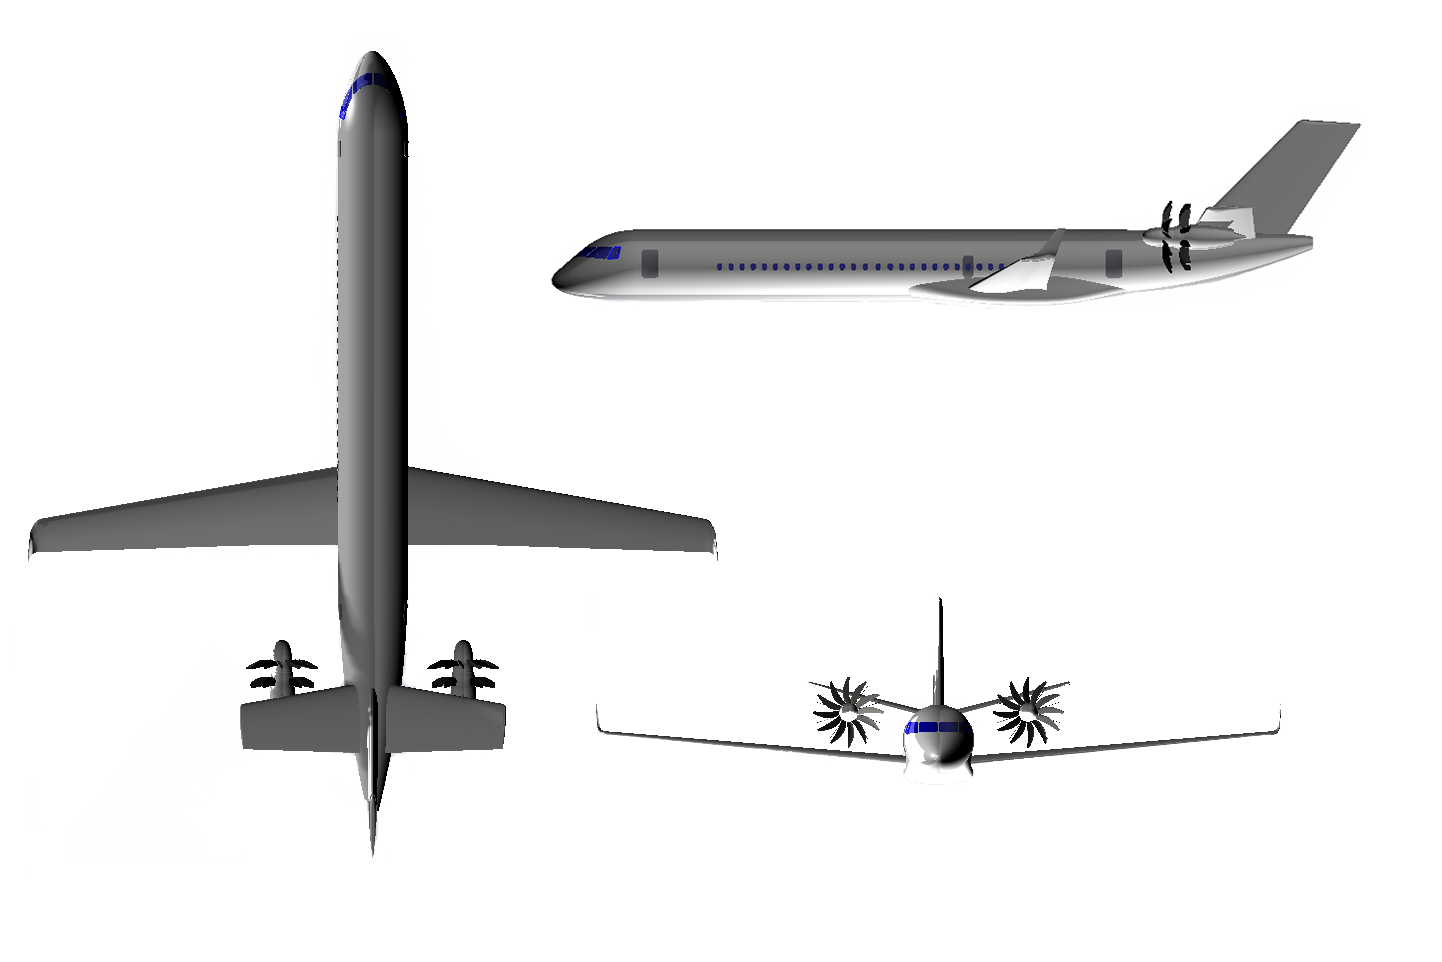
\includegraphics[height=10.5cm, keepaspectratio ]{Immagini/Capitolo3/IRON} 
	\caption{Layout of Regional Turboprop. Side, top and front section.} % didascalia
	\label{fig:figura3_0} % etichetta per citarla nel testo
\end{figure}

\begin{figure}[H]
	\centering
	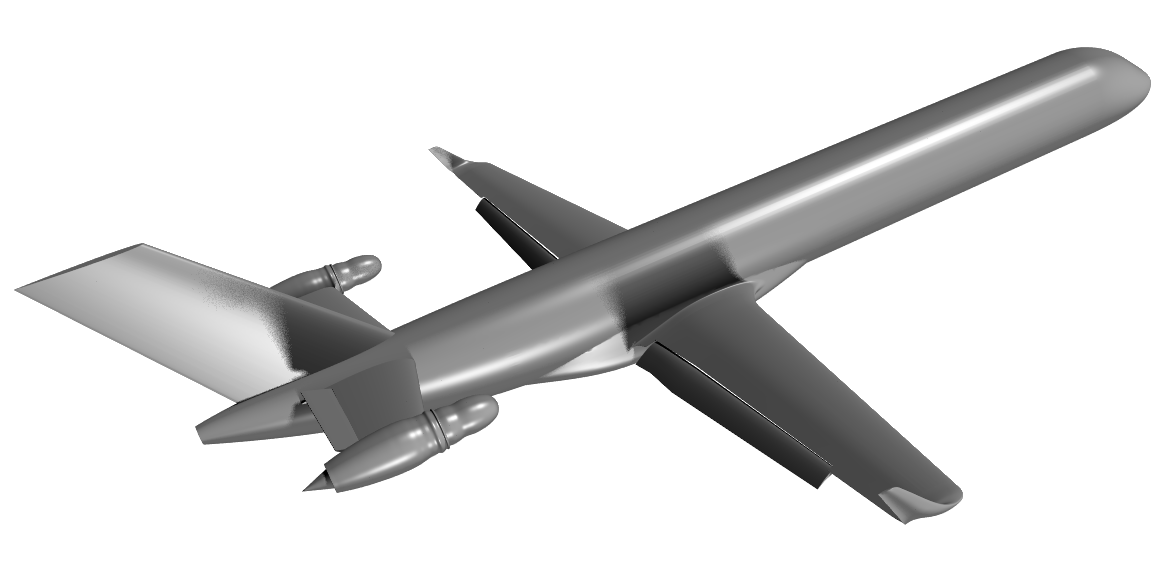
\includegraphics[height=7cm, keepaspectratio ]{Immagini/Capitolo3/IRON_TAKE_OFF} 
	\caption{Regional Turboprop rendering in takeoff configuration} % didascalia
	\label{fig:figura3_01} % etichetta per citarla nel testo
\end{figure}

\begin{table}[H]
\begin{centering}
\begin{tabular}{llc}
\toprule
\textbf{Data}&\textbf{Value} \\
\hline
\multirow{ 7}{*}{Wing}&Span	&	35.34 m	\\
& AR & 12 \\
& $C_r$ & 5.325 m \\
& $C_k$ & 4.5 m \\
& $C_t$ & 3.4 m \\
&  MAC & 3.16 m \\
& Flap type & FOWLER \\
& $\delta_{f_{TO}}$ & $\ang{25}$ \\
\hline
\multirow{4}{*}{Horizontal Tail }&Span	&	12.5 m	\\
& $C_r$ & 3.64 m \\
& $C_t$ & 2.272 m \\
& $\delta_{e_{min}}$ & $\ang{-25}$ \\
\hline
Other data&MTOW	&	51847 kg	\\
\bottomrule

\end{tabular}
\caption{Aircraft main data.}
\label{tabellaB.1}
\end{centering}
\end{table}


\begin{figure}[H]
	%\centering
	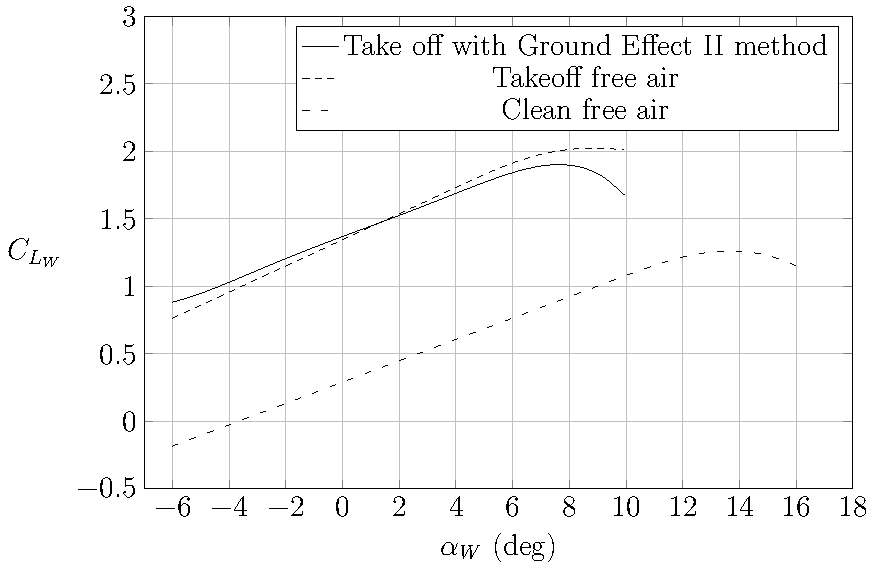
\includegraphics[height=9.5cm, keepaspectratio ]{Immagini/Capitolo3/3_1-GroundEffectOnWingLiftCurve} 
	\caption{Ground effect on wing lift curve} % didascalia
	\label{fig:figura3_1} % etichetta per citarla nel testo
\end{figure}

\begin{figure}[H]
	%\centering
	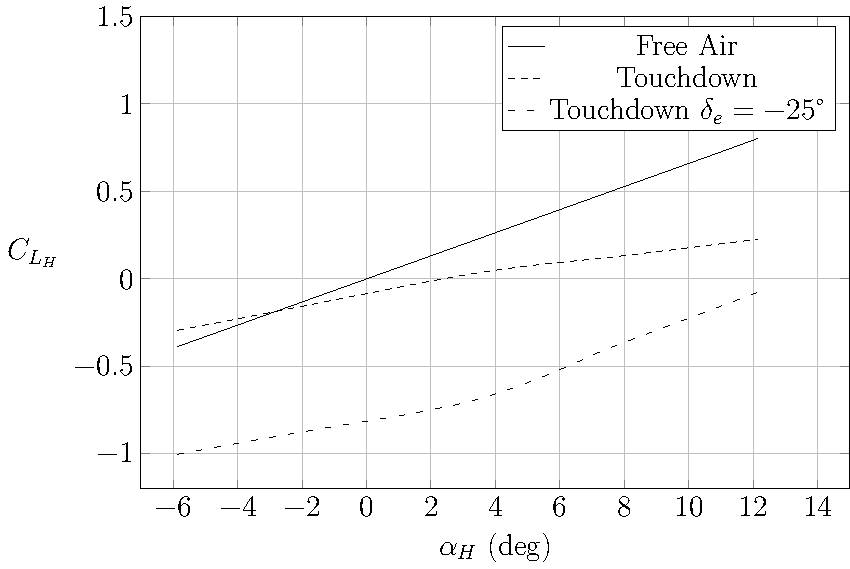
\includegraphics[height=9.5cm, keepaspectratio ]{Immagini/Capitolo3/3_2-GroundEffectOnHorizontalTailLiftCurve} 
	\caption{Ground effect on horizontal tail lift curve} % didascalia
	\label{fig:figura3_2} % etichetta per citarla nel testo
\end{figure}

\begin{figure}[H]
	%\centering
	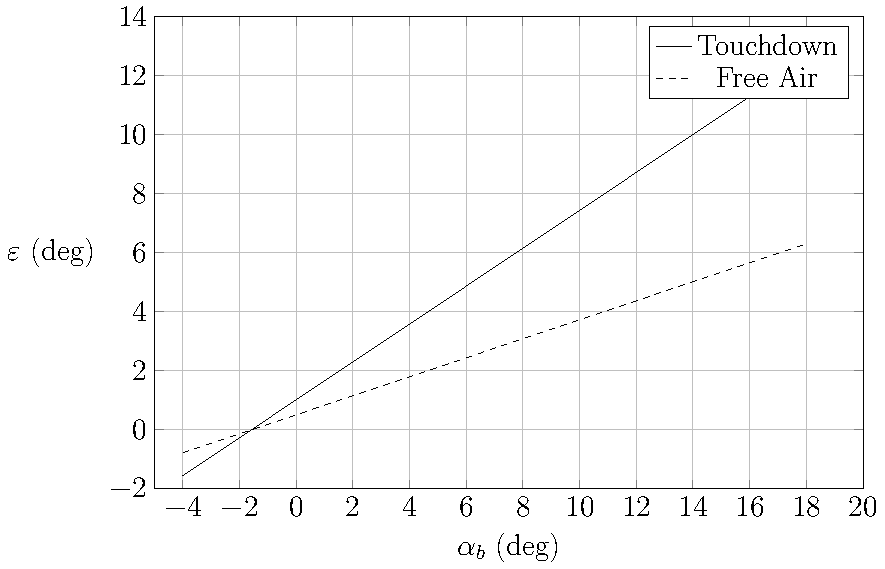
\includegraphics[height=9cm, keepaspectratio ]{Immagini/Capitolo3/3_3-GroundEffectOnDownwashAngle} 
	\caption{Ground effect on downwash angle} % didascalia
	\label{fig:figura3_3} % etichetta per citarla nel testo
\end{figure}

\begin{figure}[H]
	%\centering
	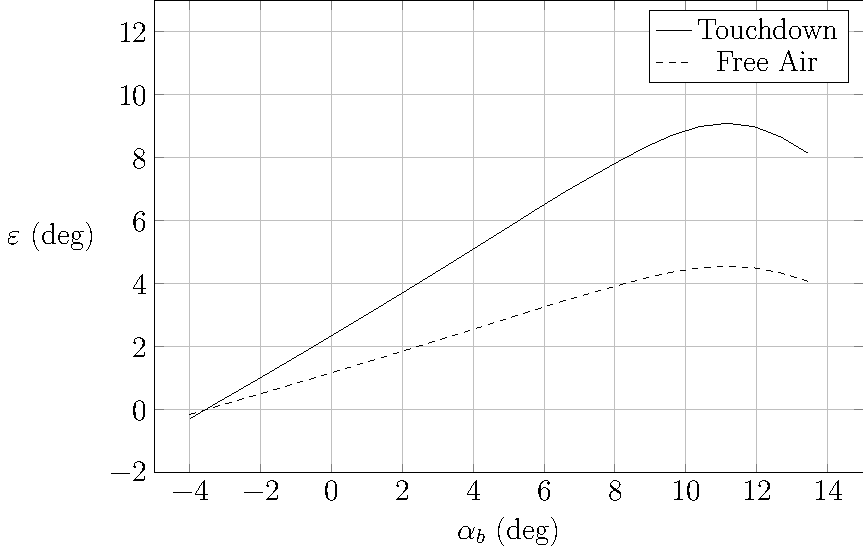
\includegraphics[height=9cm, keepaspectratio ]{Immagini/Capitolo3/3_4-GroundEffectOnDownwashAngleConsideringNonLinearEffects} 
	\caption{Ground effect on downwash angle considering non linear effects} % didascalia
	\label{fig:figura3_4} % etichetta per citarla nel testo
\end{figure} 

% -----------------------------------------------------------------------------------------
%                                                                 APPENDICI
% -----------------------------------------------------------------------------------------

\appendix

\chapter{HDF dataset and database reader creation}
\label{ch:hdigitalizer}
\markboth{HDF dataset and database reader creation}{}
In a tool for preliminary design phase of an aircraft, it's very important to have aviable database. It's possible to create database starting from graphics using external software. In this appendix will be explained the step required in order to digitalize the graphics, create an HDF dataset and set up the database-reader class in Jpad.

\section{Chart Digitization}
The first step required for create a dataset is to digitalize a chart. Often data is found presented in reports and references as functional X-Y type scatter or line plots. In order to use this data, it must somehow be digitized. This is made with an external software, such as {\itshape Plot Digitizer}. Plot Digitizer is a Java program used to digitize scanned plots of functional data. This program will allow you to take a scanned image of a plot (in GIF, JPEG, or PNG format) and quickly digitize values off the plot just by clicking the mouse on each data point.\cite{plotdigitizer}

\begin{figure}[H]
\centering
{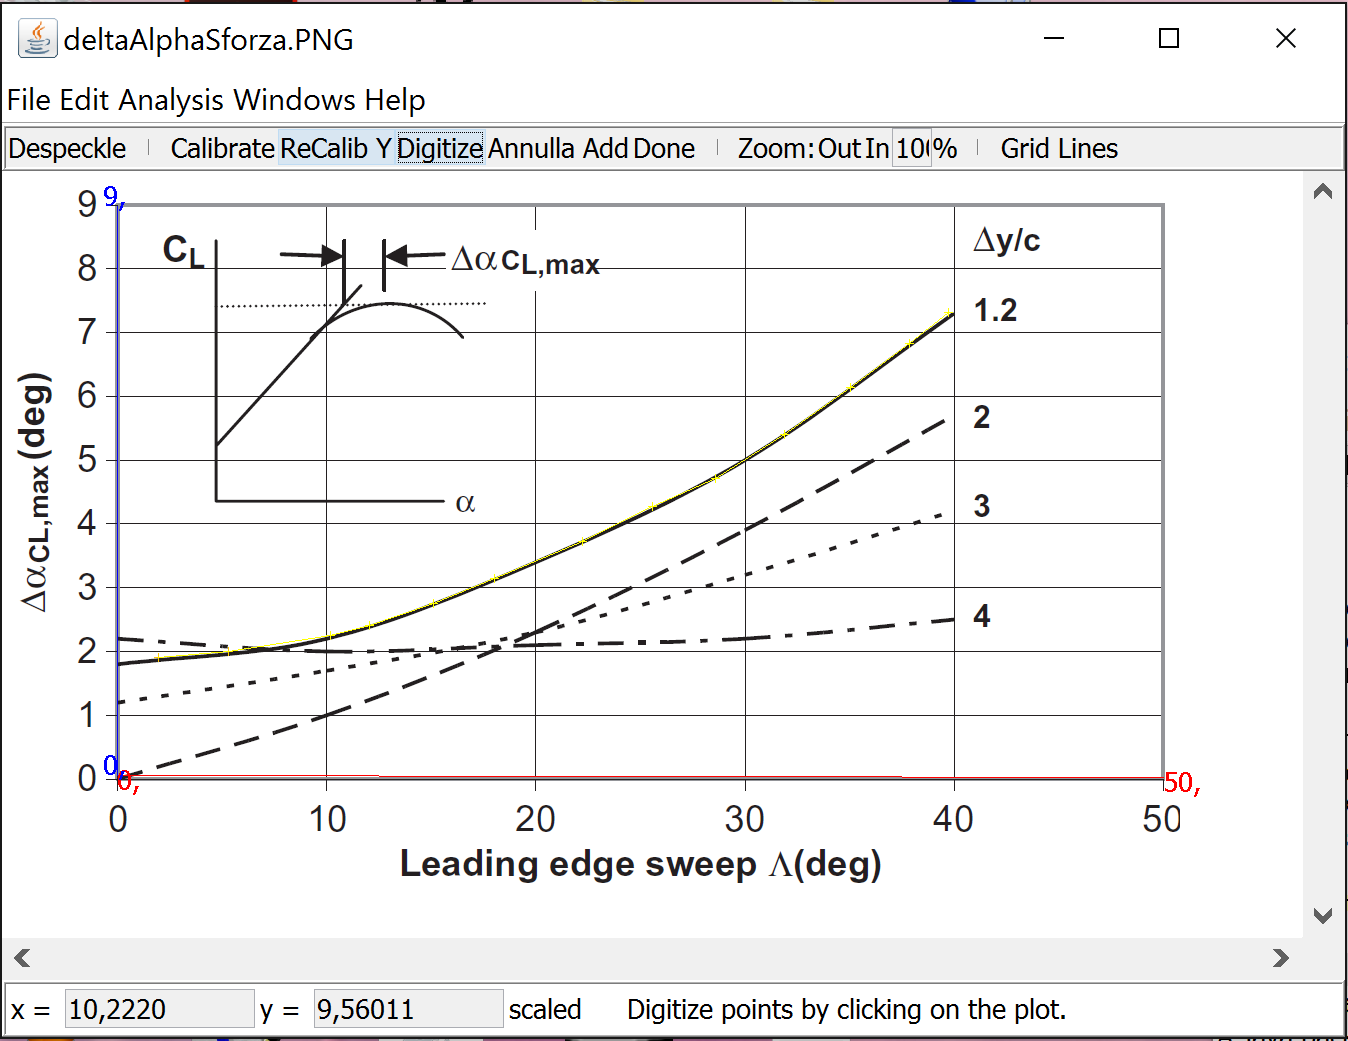
\includegraphics[height=7.9cm]{Immagini/digitize.png}} 
\caption{Chart digitization using Plot Digitizer.}
\label{angles}
\end{figure} 


In order to digitize a chart, first of all it's necessary to calibrate the axis. Plot Digitizer works with both linear and logarithmic axis scales. After it's possible to digitize a curve simply click o it. The values obtained can then be saved to a tex file or .csv file.


\section{Creation of an HDF file with Matlab}

Obtained the .csv file from digitization is necessary to create the HDF file. First of all it's necessary to import the file with couple of coordinates as matrix. After saving the imported files as .mat file, Matlab code comes in play to manage these data and to generate the digitalized curves and the HDF dataset.  The code interpolates curves points with cubic splines in order to have more points to plot for each curve.

\bigskip
\lstset{language=Matlab}
\begin{lstlisting}[frame=rbl,caption={{\footnotesize MATLAB script for creating the HDF Database}},label= [style=\bfseries]{Listing}]
clc; close all; clear all;

%% Import data
DeltaAlphaCLmax_vs_LambdaLE_dy1p2 = importdata('DeltaAlphaCLmax_vs_LambdaLE_dy1p2.mat');
DeltaAlphaCLmax_vs_LambdaLE_dy2p0 = importdata('DeltaAlphaCLmax_vs_LambdaLE_dy2p0.mat');
DeltaAlphaCLmax_vs_LambdaLE_dy3p0 = importdata('DeltaAlphaCLmax_vs_LambdaLE_dy3p0.mat');
DeltaAlphaCLmax_vs_LambdaLE_dy4p0 = importdata('DeltaAlphaCLmax_vs_LambdaLE_dy4p0.mat');

nPoints = 30;
lambdaLEVector_deg = transpose(linspace(0, 40, nPoints));

%% dy/c = 1.2
smoothingParameter = 0.999999;
DAlphaVsLambdaLESplineStatic_Dy1p2 = csaps( ...
    DeltaAlphaCLmax_vs_LambdaLE_dy1p2(:,1), ...
    DeltaAlphaCLmax_vs_LambdaLE_dy1p2(:,2), ...
    smoothingParameter ...
    );

DAlphaVsLambdaLEStatic_Dy1p2 = ppval( ...
    DAlphaVsLambdaLESplineStatic_Dy1p2, ...
    lambdaLEVector_deg ...
    );

%% dy/c = 2.0

smoothingParameter = 0.999999; 
DAlphaVsLambdaLESplineStatic_Dy2p0 = csaps( ...
    DeltaAlphaCLmax_vs_LambdaLE_dy2p0(:,1), ...
    DeltaAlphaCLmax_vs_LambdaLE_dy2p0(:,2), ...
    smoothingParameter ...
    );

DAlphaVsLambdaLEStatic_Dy2p0 = ppval( ...
    DAlphaVsLambdaLESplineStatic_Dy2p0, ...
    lambdaLEVector_deg ...
    );

%% dy/c = 3.0

smoothingParameter =0.999999;
DAlphaVsLambdaLESplineStatic_Dy3p0 = csaps( ...
    DeltaAlphaCLmax_vs_LambdaLE_dy3p0(:,1), ...
    DeltaAlphaCLmax_vs_LambdaLE_dy3p0(:,2), ...
    smoothingParameter ...
    );

DAlphaVsLambdaLEStatic_Dy3p0 = ppval( ...
    DAlphaVsLambdaLESplineStatic_Dy3p0, ...
    lambdaLEVector_deg ...
    );

%% dy/c = 4.0

smoothingParameter = 0.999999; 
DAlphaVsLambdaLESplineStatic_Dy4p0 = csaps( ...
    DeltaAlphaCLmax_vs_LambdaLE_dy4p0(:,1), ...
    DeltaAlphaCLmax_vs_LambdaLE_dy4p0(:,2), ...
    smoothingParameter ...
    );

DAlphaVsLambdaLEStatic_Dy4p0 = ppval( ...
    DAlphaVsLambdaLESplineStatic_Dy4p0, ...
    lambdaLEVector_deg ...
    );


%% Plots
figure(1)
plot ( ...
    lambdaLEVector_deg, DAlphaVsLambdaLEStatic_Dy1p2, '-*b' ... , ...
 );
 hold on
 
 plot ( ...
    lambdaLEVector_deg, DAlphaVsLambdaLEStatic_Dy2p0, '-b' ... , ...
 );

hold on

plot ( ...
    lambdaLEVector_deg, DAlphaVsLambdaLEStatic_Dy3p0, '*b' ... , ...
 );

hold on

plot ( ...
    lambdaLEVector_deg, DAlphaVsLambdaLEStatic_Dy4p0, 'b' ... , ...
 );

 xlabel('\Lambda_{le} (deg)'); ylabel('\Delta\alpha_{C_{L,max}}');
 title('Angle of attack increment for wing maximum lift in subsonic flight');
  legend('\Delta y/c = 1.2', '\Delta y/c = 2.0', '\Delta y/c = 3.0','\Delta y/c = 4.0');
 axis([0 50 0 9]);
 grid on;
 

 
%% preparing output to HDF

% dy/c
dyVector = [ ...
    1.2;2.0;3.0;4.0 ...
    ];

%columns --> curves
myData = [ ...
    DAlphaVsLambdaLEStatic_Dy1p2,...
        DAlphaVsLambdaLEStatic_Dy2p0, ... % -> 2
        DAlphaVsLambdaLEStatic_Dy3p0, ... % -> 3
        DAlphaVsLambdaLEStatic_Dy4p0];    % -> 4

hdfFileName = 'DAlphaVsLambdaLEVsDy.h5';

if ( exist(hdfFileName, 'file') )
    fprintf('file %s exists, deleting and creating a new one\n', hdfFileName);
    delete(hdfFileName)
else
    fprintf('Creating new file %s\n', hdfFileName);
end

% Dataset: data
h5create(hdfFileName, '/DAlphaVsLambdaLEVsDy/data', size(myData'));
h5write(hdfFileName, '/DAlphaVsLambdaLEVsDy/data', myData');

% Dataset: var_0
h5create(hdfFileName, '/DAlphaVsLambdaLEVsDy/var_0', size(dyVector'));
h5write(hdfFileName, '/DAlphaVsLambdaLEVsDy/var_0', dyVector');

% Dataset: var_1
h5create(hdfFileName, '/DAlphaVsLambdaLEVsDy/var_1', size(lambdaLEVector_deg'));
h5write(hdfFileName, '/DAlphaVsLambdaLEVsDy/var_1', lambdaLEVector_deg');
\end{lstlisting}

\noindent \\ \\ 
This script plot the graph after digitization. In this way it's possible to compare the initial graph and the digitized one.


 \begin{figure}[H]
\centering
{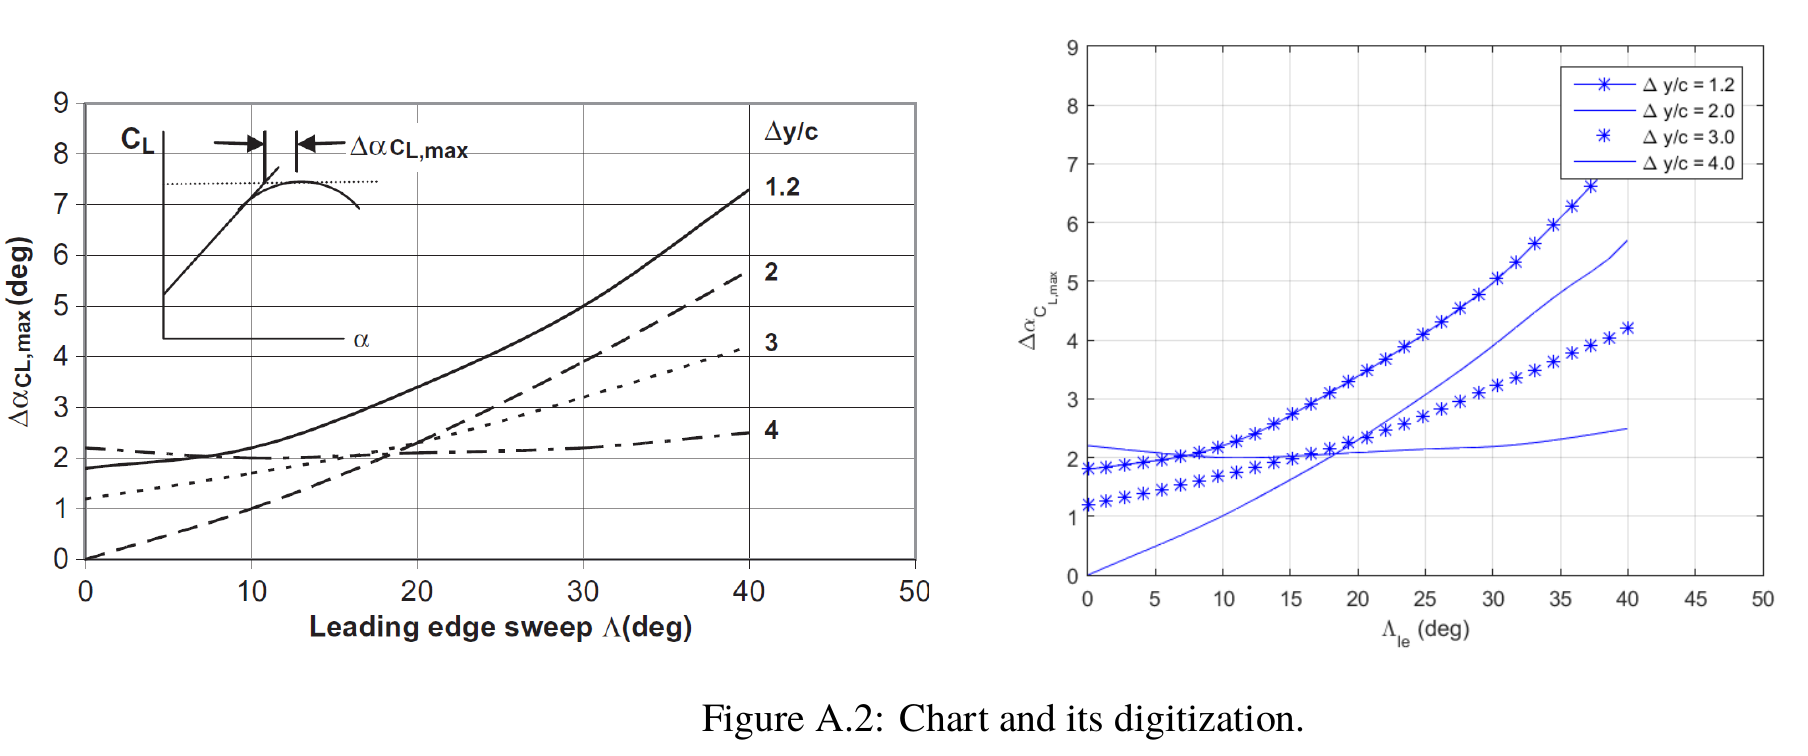
\includegraphics[height=6cm]{Immagini/digitize2.png}} 
\label{angles}
\end{figure} 





%-------------------------------------------------------------------------------------------

\thispagestyle{empty} % per non inserire una pagina nella numerazione

% -----------------------------------------------------------------------------------------
%                                                               B I B L I O G R A F I A
% -----------------------------------------------------------------------------------------
\thispagestyle{empty}
\printbibliography[heading=bibintoc]

\end{document}
